% TEMPLATE for Usenix papers, specifically to meet requirements of
%  USENIX '05
% originally a template for producing IEEE-format articles using LaTeX.
%   written by Matthew Ward, CS Department, Worcester Polytechnic Institute.
% adapted by David Beazley for his excellent SWIG paper in Proceedings,
%   Tcl 96
% turned into a smartass generic template by De Clarke, with thanks to
%   both the above pioneers
% use at your own risk.  Complaints to /dev/null.
% make it two column with no page numbering, default is 10 point

% Munged by Fred Douglis <douglis@research.att.com> 10/97 to separate
% the .sty file from the LaTeX source template, so that people can
% more easily include the .sty file into an existing document.  Also
% changed to more closely follow the style guidelines as represented
% by the Word sample file. 
% This version uses the latex2e styles, not the very ancient 2.09 stuff.
\documentclass[letterpaper,twocolumn,10pt]{article}
\usepackage{usenix,epsfig,endnotes,xspace,color}

% Name candidates:
%  Anza
%  Void 
%  Station (from Genesis's Grand Central component) 
%  TARDIS: Atomic, Recoverable, Datamodel Independent Storage
% EAB: flex, basis, stable, dura
% Stasys:  SYStem for Adaptable Transactional Storage: 

\newcommand{\yad}{Stasis\xspace}
\newcommand{\yads}{Stasis'\xspace}
\newcommand{\oasys}{Oasys\xspace}

%\newcommand{\graphdbg}[1]{\fbox{#1}}
\newcommand{\graphdbg}[1]{#1}

\newcommand{\diff}[1]{\textcolor{blue}{\bf #1}}
\newcommand{\eab}[1]{\textcolor{red}{\bf EAB: #1}}
\newcommand{\rcs}[1]{\textcolor{green}{\bf RCS: #1}}
%\newcommand{\mjd}[1]{\textcolor{blue}{\bf MJD: #1}}

\newcommand{\eat}[1]{}

\renewcommand\figurename{\sf \small Figure}

\begin{document}

%don't want date printed
\date{}


%make title bold and 14 pt font (Latex default is non-bold, 16 pt)

\title{\Large \bf \yad: System for Adaptable, Transactional Storage}

%for single author (just remove % characters)
\author{
{\rm Russell Sears}\\
UC Berkeley
\and
{\rm Eric Brewer}\\
UC Berkeley
\vspace*{-.25in}
} % end author

\maketitle

% Use the following at camera-ready time to suppress page numbers.
% Comment it out when you first submit the paper for review.
\thispagestyle{empty}

%\abstract
%\subsection*{Abstract}
\rcs{Spell check, look at end notes and figure captions.  Spell check / cannonicalize bibtex.  Embed graph fonts.}

{\em An increasing range of applications requires robust support for atomic, durable and concurrent
transactions.  Databases provide the default solution, but force
applications to interact via SQL and to forfeit control over data
layout and access mechanisms.  We argue there is a gap between DBMSs and file systems that limits designers of data-oriented applications.

\yad is a storage framework that incorporates ideas from traditional
write-ahead logging algorithms and file systems.
It provides applications with flexible control over data structures, data layout, robustness, and performance.
\yad enables the development of
unforeseen variants on transactional storage by generalizing
write-ahead logging algorithms.  Our partial implementation of these
ideas already provides specialized (and cleaner) semantics to applications.

We evaluate the performance of a traditional transactional storage
system based on \yad, and show that it performs favorably relative to existing
systems.  We present examples that make use of custom access methods, modified
buffer manager semantics, direct log file manipulation, and LSN-free
pages.  These examples facilitate sophisticated performance 
optimizations such as zero-copy I/O.  These extensions are composable,
easy to implement and significantly improve performance.

}
%We argue that our ability to support such a diverse range of
%transactional systems stems directly from our rejection of
%assumptions made by early database designers.  These assumptions
%permeate ``database toolkit'' research.  We attribute the success of
%low-level transaction processing libraries (such as Berkeley DB) to
%a partial break from traditional database dogma.

% entries, and 
% to reduce memory and
%CPU overhead, reorder log entries for increased efficiency, and do
%away with per-page LSNs in order to perform zero-copy transactional
%I/O.  
%We argue that encapsulation allows applications to compose
%extensions.

%These ideas have been partially implemented, and initial performance
%figures, and experience using the library compare favorably with
%existing systems.



\section{Introduction}
\label{sec:intro}
As our reliance on computing infrastructure increases, a wider range
of applications requires robust data management.  Traditionally, data
management has been the province of database management systems
(DBMSs), which are well-suited to enterprise applications, but lead to
poor support for systems such as web services, search engines, version
systems, work-flow applications, bioinformatics, and
scientific computing.  These applications have complex transactional
storage requirements, but do not fit well onto SQL or the monolithic
approach of current databases.  In fact, when performance matters
these applications often avoid DBMSs and instead implement ad-hoc data
management solutions~\cite{mapReduce,SNS}.

An example of this mismatch occurs with DBMS support for persistent objects.
In a typical usage, an array of objects is made persistent by mapping
each object to a row in a table (or sometimes multiple
tables)~\cite{hibernate} and then issuing queries to keep the objects
and rows consistent. 
%An update must confirm it has the current
%version, modify the object, write out a serialized version using the
%SQL update command, and commit.  
Also, for efficiency, most systems
must buffer two copies of the application's working set in memory.
This is an awkward and inefficient mechanism, and hence we claim that
DBMSs do not support this task well.

Search engines and data warehouses in theory can use the relational
model, but in practice need a very different implementation.
Object-oriented, XML, and streaming databases all have distinct
conceptual models and underlying implementations.

Scientific computing, bioinformatics and version-control systems tend
to preserve old versions and track provenance.  Thus they each have a
distinct conceptual model.  Bioinformatics systems perform
computations over large, semi-structured databases.  Relational
databases support none of these requirements well. Instead, office
suites, ad-hoc text-based formats and Perl scripts are used for data
management~\cite{perl}, with mixed success~\cite{excel}.

Our hypothesis is that 1) each of these areas has a distinct top-down
conceptual model (which may not map well to the relational model); and
2) there exists a bottom-up layered framework that can better support
all of these models and others.

To explore this hypothesis, we present \yad, a library that provides
transactional storage at a level of abstraction as close to the
hardware as possible.  It can support special-purpose
transactional storage models in addition to ACID database-style
interfaces to abstract data models.  \yad incorporates techniques from both
databases (e.g. write-ahead logging) and operating systems
(e.g. zero-copy techniques).

Our goal is to combine the flexibility and layering of low-level
abstractions typical for systems work with the complete semantics
that exemplify the database field.
By {\em flexible} we mean that \yad{}  can support a wide
range of transactional data structures {\em efficiently}, and that it can support a variety
of policies for locking, commit, clusters and buffer management.
Also, it is extensible for new core operations
and data structures. This flexibility allows it to
support a wide range of systems and models.

By {\em complete} we mean full redo/undo logging that supports
both {\em no force}, which provides durability with only log writes,
and {\em steal}, which allows dirty pages to be written out prematurely
to reduce memory pressure. By complete, we also
mean support for media recovery, which is the ability to roll
forward from an archived copy, and support for error-handling,
clusters, and multithreading. These requirements are difficult
to meet and form the {\em raison d'\^etre} for \yad{}: the framework
delivers these properties as reusable building blocks for systems
that implement complete transactions.

Through examples and their good performance, we show how \yad{}
efficiently supports a wide range of uses that fall in the gap between 
database and file system technologies, including
persistent objects, graph- or XML-based applications, and recoverable
virtual memory~\cite{lrvm}.  

For example, on an object persistence workload, we provide up to 
a 4x speedup over an in-process MySQL implementation and a 3x speedup over Berkeley DB, while 
cutting memory usage in half (Section~\ref{sec:oasys}). 
We implemented this extension in 150 lines of C, including comments and boilerplate.  We did not have this type of optimization
in mind when we wrote \yad, and in fact the idea came from a
user unfamiliar with \yad.

%\e ab{others?  CVS, windows registry, berk DB, Grid FS?}
%\r cs{maybe in related work?}

This paper begins by contrasting \yads approach with that of
conventional database and transactional storage systems.  It proceeds
to discuss write-ahead logging, and describe ways in which \yad can be
customized to implement many existing (and some new) write-ahead
logging variants.  We present implementations of some of these variants and
benchmark them against popular real-world systems.  We
conclude with a survey of related and future work.
An (early) open-source implementation of
the ideas presented here is available (see Section~\ref{sec:avail}).

\section{\yad is not a Database}
\label{sec:notDB}

Database research has a long history, including the development of
many of the technologies we exploit.  This section explains
why databases are fundamentally inappropriate tools for system
developers, and covers some of the previous responses of the systems
community.  These problems have been the focus of
database and systems researchers for at least 25 years.

\subsection{The Database View}

The database community approaches the limited range of DBMSs by either
creating new top-down models, such as object-oriented, XML or streaming databases~\cite{streaming, XMLdb},
or by extending the relational model~\cite{codd} along some axis, such
as new data types~\cite{newDBtypes}.  We cover these attempts in more detail in
Section~\ref{sec:related-work}.

%Database systems are often thought of in terms of the high-level
%abstractions they present.  For instance, relational database systems
%implement the relational model~\cite{codd}, object-oriented
%databases implement object abstractions \eab{[?]}, XML databases implement
%hierarchical datasets~\eab{[?]}, and so on.  Before the relational model,
%navigational databases implemented pointer- and record-based data models.

An early survey of database implementations sought to enumerate the
fundamental components used by database system implementors~\cite{batoryConceptual,batoryPhysical}.  This
survey was performed due to difficulties in extending database systems
into new application domains.  It divided internal database
routines into two broad modules: {\em conceptual mappings} and {\em physical
database models}.
%A physical model would then translate a set of tuples into an
%on-disk B-tree, and provide support for iterators and range-based query
%operations.
It is the responsibility of a database implementor to choose a set of
conceptual mappings that implement the desired higher-level
abstraction (such as the relational model).  The physical data model
is chosen to support efficiently the set of mappings that are built on
top of it.

A conceptual mapping based on the relational model might translate a
relation into a set of keyed tuples.  If the database were going to be
used for short, write-intensive and high-concurrency transactions
(OLTP), the physical model would probably translate sets of tuples
into an on-disk B-tree.  In contrast, if the database needed to
support long-running, read-only aggregation queries (OLAP) over high-dimensional data, a physical model that stores the data in a sparse
array format would be more appropriate~\cite{OLAP,molap}.  Although both
OLTP and OLAP databases are based upon the relational model they make
use of different physical models in order to serve
different classes of applications efficiently.  

A basic claim of this paper is that no known physical data model can
efficiently support the wide range of conceptual mappings that are in
use today.  In addition to sets, objects, and XML, such a model would
need to cover search engines, version-control systems, work-flow
applications, and scientific computing, as examples.  Similarly, a
recent database paper argues that the "one size fits all" approach of
DBMSs no longer works~\cite{oneSizeFitsAll}.

Instead of attempting to create such a unified model after decades of
database research has failed to produce one, we opt to provide a
bottom-up transactional toolbox that supports many models
efficiently.  This makes it easy for system designers to
implement most data models that the underlying hardware can
support, or to abandon the database approach entirely, and forgo 
%structured physical models and abstract conceptual mappings.
a top down model.

\subsection{The Systems View}
\label{sec:systems}

The systems community has also worked on this mismatch, which has led
to many interesting projects.  Examples include alternative durability
models such as QuickSilver~\cite{experienceWithQuickSilver},
RVM~\cite{lrvm}, persistent objects~\cite{argus}, and persistent data structures~\cite{DDS,boxwood}.  We expect that \yad
would simplify the implementation of most if not all of these systems.
Section~\ref{sec:related-work} covers these in more detail.

In some sense, our hypothesis is trivially true in that there exists a
bottom-up framework called the ``operating system'' that can implement
all of the models. A famous database paper argues that it does so
poorly (Stonebraker 1981~\cite{Stonebraker81}). Our task is really to
simplify the implementation of transactional systems through more
powerful primitives that enable concurrent transactions with a variety
of performance/robustness tradeoffs.

The closest system to ours in spirit is Berkeley DB,  a highly successful alternative to conventional
databases~\cite{libtp}.  At its core, it provides the physical database model
(relational storage system~\cite{systemR}) of a conventional database server.
%It is based on the
%observation that the storage subsystem is a more general (and less
%abstract) component than a monolithic database, and provides a
%stand-alone implementation of the storage primitives built into 
%most relational database systems~\cite{libtp}.  
In particular, 
it provides transactional (ACID) operations on B-trees, 
hash tables, and other access methods.  It provides flags that 
let its users tweak aspects of the performance of these
primitives, and selectively disable the features it provides.

With the exception of the benchmark designed to compare the two
systems, none of the \yad applications presented in
Section~\ref{experiments} are efficiently supported by Berkeley DB.
This is a result of Berkeley DB's assumptions regarding workloads and
low-level data representations.  Thus, although
Berkeley DB could be built on top of \yad, Berkeley DB's data model
and write-ahead logging system are too specialized to support \yad.




\section{Transactional Pages}

\rcs{still missing refs to PhDs on layering}

This section describes how \yad implements transactions that are
similar to those provided by relational database systems, which are
based on transactional pages.  The algorithms described in this
section are not novel, and are in fact based on
ARIES~\cite{aries}.  However, they form the starting point for
extensions and novel variants, which we cover in the next two
sections.

As with other systems, \yads transactions have a two-level structure.
The lower level of an operation provides atomic updates to regions of
the disk.  These updates do not have to deal with concurrency, but
must update the page file atomically, even if the system crashes.

The higher level provides operations that span multiple pages by
atomically applying sets of operations to the page file and coping
with concurrency issues.  Surprisingly, the implementations of these
two layers are only loosely coupled.


\subsection{Atomic Disk Operations}

Transactional storage algorithms work by
atomically updating portions of durable storage.  These small atomic
updates bootstrap transactions that are too large to be
applied atomically.  In particular, write-ahead logging (and therefore
\yad) relies on the ability to write entries to the log
file atomically.  Transaction systems that store sequence numbers on pages to 
track version information also rely on atomic page writes. 

In practice, a write to a disk page is not atomic (in modern drives).  Two common failure
modes exist.  The first occurs when the disk writes a partial sector
during a crash.  In this case, the drive maintains an internal
checksum, detects a mismatch, and reports it when the page is read.
The second case occurs because pages span multiple sectors.  Drives
may reorder writes on sector boundaries, causing an arbitrary subset
of a page's sectors to be updated during a crash.  {\em Torn page
detection} can be used to detect this phenomenon, typically by
requiring a checksum for the whole page. 

Torn and corrupted pages may be recovered by using {\em media
recovery} to restore the page from backup.  Media recovery works by
reloading the page from an archive copy, and bringing it up to date by
replaying the log.

For simplicity, this section ignores mechanisms that detect
and restore torn pages, and assumes that page writes are atomic.
We relax this restriction in Section~\ref{sec:lsn-free}.

\subsection{Non-concurrent Transactions}

This section provides the ``Atomicity'' and ``Durability'' properties
for a single ACID transaction.\endnote{The ``A'' in ACID really means ``atomic persistence
of data,'' rather than ``atomic in-memory updates,'' as the term is normally
used in systems work; the latter is covered by ``C'' and ``I''~\cite{GR97}.}
First we describe single-page transactions, then multi-page transactions.
``Consistency'' and ``Isolation'' are covered with 
concurrent transactions in the next section.
%We cover
%multi-page transactions in the next section, and the rest of ACID in
%Section~\ref{locking}.  

The insight behind transactional pages was
that atomic page writes form a good foundation for full transactions.
However, since page writes are no longer atomic, it might be
better to think of these as transactional sectors.

The trivial way to achieve single-page transactions is to apply all of
the updates to the page and then write it out on commit.  The page
must be pinned until commit to prevent write-back of uncommitted data,
but no logging is required.

This approach performs poorly because we {\em force} the page to disk
on commit, which leads to a large number of synchronous non-sequential
writes.  By writing redo information to the log before committing
(write-ahead logging), we get {\em no force} transactions and better
performance, since the synchronous writes to the log are sequential.
Later, the pages are written out asynchronously, often
as part of a larger sequential write.

After a crash, we have to apply the redo entries to those pages that
were not updated on disk.  To decide which updates to reapply, we use
a per-page version number called the {\em log-sequence number} or
{\em LSN}. Each update to a page increments the LSN, writes it on the
page, and includes it in the log entry.  On recovery, we 
load the page, use the LSN to figure out which updates are missing
(those with higher LSNs), and reapply them.

Updates from aborted transactions should not be applied, so we also
need to log commit records; a transaction commits when its commit
record correctly reaches the disk. Recovery starts with an analysis
phase that determines all of the outstanding transactions and their
fate.  The redo phase then applies the missing updates for committed
transactions.

Pinning pages until commit also hurts performance, and could even
affect correctness if a single transaction needs to update more pages
than can fit in memory. A related problem is that with concurrency a
single page may be pinned forever as long as it has at least one
active transaction in progress all the time.  Systems that support
{\em steal} avoid these problems by allowing pages to be written back
early.  This implies we may need to undo updates on the page if the
transaction aborts, and thus before we can write out the page we must
write the undo information to the log. 

On recovery, the redo phase applies all updates (even those from
aborted transactions).  Then, an undo phase corrects stolen pages for
aborted transactions.  Each operation that undo performs is recorded
in the log, and the per-page LSN is updated accordingly.  In order to
ensure progress even with crashes during recovery, special log records
mark which actions have been undone, so they may be skipped during
recovery in the future.  We also use these records, called {\em
Compensation Log Records (CLRs)} to avoid undoing actions that we
intend to keep even when transactions abort.

The primary difference between \yad and ARIES for basic transactions
is that \yad allows user-defined operations, while ARIES defines a set
of operations that support relational database systems.  An {\em
operation} consists of an undo and a redo function.  Each time an
operation is invoked, a corresponding log entry is generated.  We
describe operations in more detail in Section~\ref{sec:operations}

%\subsection{Multi-page Transactions}

Given steal/no-force single-page transactions, it is relatively easy
to build full transactions. 
To recover a multi-page transaction, we simply recover each of
the pages individually.  This works because steal/no-force completely
decouples the pages: any page can be written back early (steal) or
late (no force).  

\subsection{Concurrent Transactions}
\label{sec:nta}

Two factors make it more complicated to write operations that may be
used in concurrent transactions.  The first is familiar to anyone that
has written multi-threaded code: Accesses to shared data structures
must be protected by latches (mutexes).  The second problem stems from
the fact that abort cannot simply roll back physical updates.
%concurrent transactions prevent abort from simply
%rolling back the physical updates that a transaction made.
Fortunately, it is straightforward to reduce this second,
transaction-specific problem to the familiar problem of writing
multi-threaded software. 
% In this paper, ``concurrent
%transactions'' are transactions that perform interleaved operations;
% they may also exploit parallelism in multiprocessors.

%They do not necessarily exploit the parallelism provided by
%multiprocessor systems.  We are in the process of removing concurrency
%bottlenecks in \yads implementation.}

To understand the problems that arise with concurrent transactions,
consider what would happen if one transaction, A, rearranges the
layout of a data structure.  Next, a second transaction, B,
modifies that structure and then A aborts.  When A rolls back, its
undo entries will undo the changes that it made to the data
structure, without regard to B's modifications.  This is likely to
cause corruption.

Two common solutions to this problem are {\em total isolation} and
{\em nested top actions}.  Total isolation prevents any
transaction from accessing a data structure that has been modified by
another in-progress transaction.  An application can achieve this
using its own concurrency control mechanisms, or by holding a lock on
each data structure until the end of the transaction (by performing {\em strict two-phase locking} on the entire data structure).  
Releasing the
lock after the modification, but before the end of the transaction,
increases concurrency.  However, it means that follow-on transactions that use
the data may need to abort if this transaction aborts ({\em
cascading aborts}). 

%Related issues are studied in great detail in terms of optimistic
%concurrency control~\cite{optimisticConcurrencyControl,
%optimisticConcurrencyPerformance}.

Nested top actions avoid this problem.  The key idea is to distinguish
between the logical operations of a data structure, such as
adding an item to a set, and internal physical operations such as
splitting tree nodes. 
% We record such
%operations using {\em logical logging} and {\em physical logging},
%respectively.  
The internal operations do not need to be undone if the
containing transaction aborts; instead of removing the data item from
the page, and merging any nodes that the insertion split, we simply
remove the item from the set as application code would---we call the
data structure's {\em remove} method.  That way, we can undo the
insertion even if the nodes that were split no longer exist, or if the
data item has been relocated to a different page.  This
lets other transactions manipulate the data structure before the first
transaction commits.

In \yad, each nested top action performs a single logical operation by applying
a number of physical operations to the page file.  Physical redo and undo log entries are stored in the log so that recovery can repair any
temporary inconsistency that the nested top action introduces.  Once
the nested top action has completed, a logical undo entry is recorded,
and a CLR is used to tell recovery and abort to skip the physical
undo entries.

This leads to a mechanical approach for creating reentrant, concurrent
operations:

\begin{enumerate}
\item Wrap a mutex around each operation.  With care, it is possible 
  to use finer-grained latches in a \yad operation, but it is rarely necessary.
\item Define a {\em logical} undo for each operation (rather than a set of page-level undos).  For example, this is easy for a
  hash table: the undo for {\em insert} is {\em remove}.  The logical
  undo function should arrange to acquire the mutex when invoked by
  abort or recovery.
\item Add a ``begin nested top action'' right after mutex
  acquisition, and an ``end nested top action'' right before mutex
  release.  \yad includes operations that provide nested top
  actions.
\end{enumerate}

If the transaction that encloses a nested top action aborts, the
logical undo will {\em compensate} for the effects of the operation, 
taking updates from concurrent transactions into account.
%If a transaction should perform
%some action regardless of whether or not it commits, a nested top
%action with a ``no op'' as its inverse is a convenient way of applying
%the change.  Nested top actions do not force the log to disk, so such
%changes are not durable until the log is forced, perhaps manually, or
%by a committing transaction.  
Using this recipe, it is relatively easy to implement thread-safe
concurrent transactions.  Therefore, they are used throughout \yads
default data structure implementations.  This approach also works 
with the variable-sized atomic updates covered in Section~\ref{sec:lsn-free}.





\subsection{User-Defined Operations}
\label{sec:operations}

The first kind of extensibility enabled by \yad is user-defined operations.
Figure~\ref{fig:structure} shows how operations interact with \yad.  A
number of default operations come with \yad.  These include operations
that allocate and manipulate records, operations that implement hash
tables, and a number of methods that add functionality to recovery.
Many of the customizations described below are implemented using
custom operations. 

In this portion of the discussion, physical operations are limited to a single
page, as they must be applied atomically. Section~\ref{sec:lsn-free} removes this constraint.

Operations are invoked by registering a callback (the ``operation
implementation'' in Figure~\ref{fig:structure}) with \yad at startup,
and then calling {\tt Tupdate()} to invoke the operation at runtime.
\yad ensures that operations follow the write-ahead logging rules
required for steal/no-force transactions by controlling the timing and
ordering of log and page writes.  

The redo log entry consists of the
LSN and an argument that will be passed to redo.  The undo entry is
analogous.\endnote{For efficiency, undo and redo operations are packed
into a single log entry.  Both must take the same parameters.} Each
operation should be deterministic, provide an inverse, and acquire all
of its arguments from the argument passed via {\tt Tupdate()},
from the page it updates, or both.  The callbacks used during forward
operation are also used during recovery.  Therefore operations provide
a single redo function and a single undo function.  There is no ``do''
function, which reduces the amount of recovery-specific code in the
system.

%{\tt Tupdate()} writes the struct
%that is passed to it to the log before invoking the operation's
%implementation.  Recovery simply reads the struct from disk and
%invokes the operation at the appropriate time.

\begin{figure}
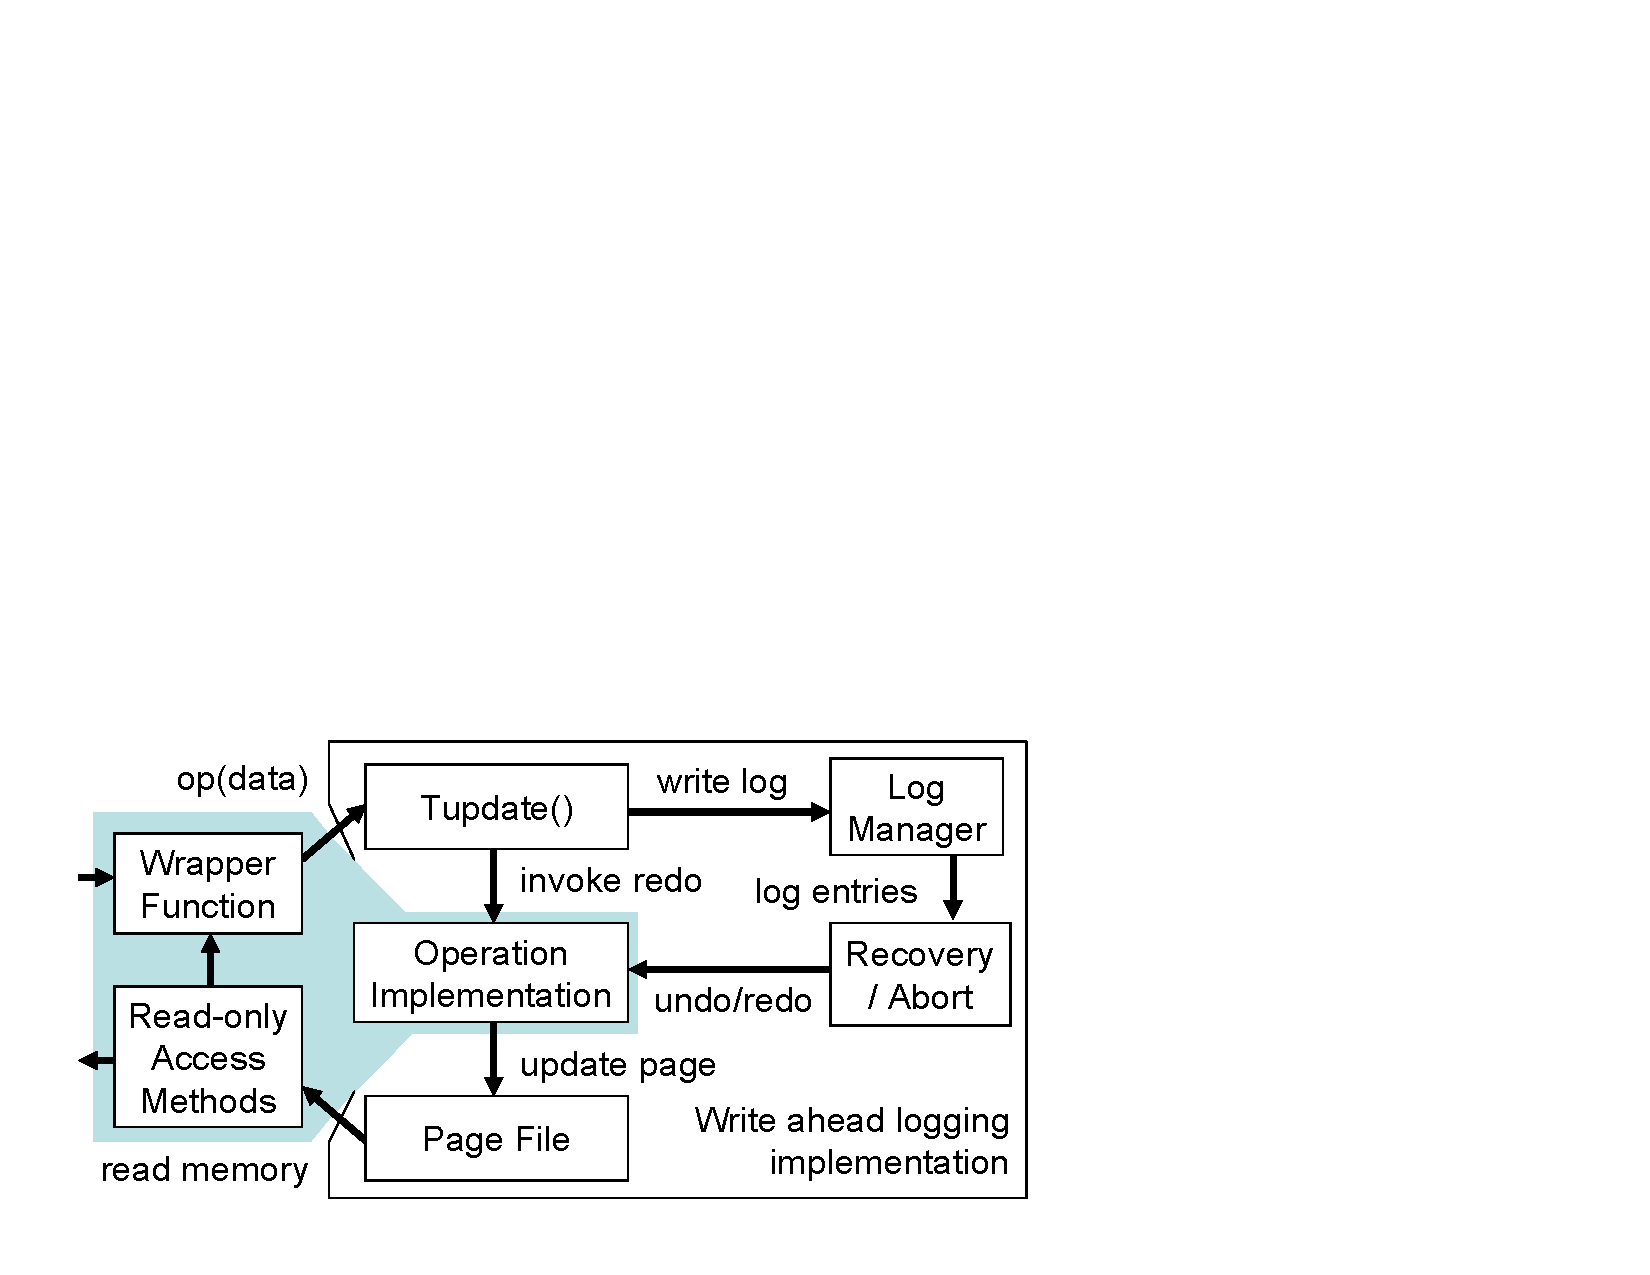
\includegraphics[%
  viewport=0bp 0bp 458bp 225bp,
  clip,
  width=1\columnwidth]{figs/structure.pdf}
{\caption{\label{fig:structure} The portions of \yad that directly interact with new operations.  The arrows point in the direction of data flow.}}
\vspace{-12pt}
\end{figure}



The first step in implementing a new operation is to decide upon an
external interface, which is typically cleaner than directly calling {\tt Tupdate()} to invoke the operation(s).
The externally visible interface is implemented
by wrapper functions and read-only access methods.  The wrapper
function modifies the state of the page file by packaging the
information that will be needed for redo/undo into a data format
of its choosing.  This data structure is passed into {\tt Tupdate()}, which writes a log entry and invokes the redo function.
 
The redo function modifies the page file directly (or takes some other
action).  It is essentially an interpreter for its log entries.  Undo
works analogously, but is invoked when an operation must be undone.

This pattern applies in many cases.  In
order to implement a ``typical'' operation, the operation's
implementation must obey a few more invariants:
\begin{itemize}
\item Pages should only be updated inside physical redo/undo operation implementations.
\item Logical operation implementations may invoke other operations
      via {\tt Tupdate()}.  Recovery does not support logical redo,
      and physical operation implementations may not invoke {\tt
      Tupdate()}.
\item The page's LSN should be updated to reflect the changes (this is
      generally handled by passing the LSN to the page implementation).

%\item If the data seen by a wrapper function must match data seen
%  during redo, then the wrapper should use a latch to protect against
%  concurrent attempts to update the sensitive data (and against
%  concurrent attempts to allocate log entries that update the data).
\item Nested top actions (and logical undo) or ``big locks'' (total isolation) should be used to manage concurrency (Section~\ref{sec:nta}).
\end{itemize}

Although these restrictions are not trivial, they are not a problem in
practice. Most read-modify-write actions can be implemented as
user-defined operations, including common DBMS optimizations such as
increment operations.  The power of \yad is that by following these
local restrictions, operations meet the global
invariants required by correct, concurrent transactions.

Finally, for some applications, the overhead of logging information for redo or
undo may outweigh their benefits.  Operations that wish to avoid undo
logging can call an API that pins the page until commit, and use an
empty undo function.  Similarly, forcing a page
to be written out on commit avoids redo logging.

\subsection{Application-specific Locking}
\label{sec:locking}
The transactions described above only provide the
``Atomicity'' and ``Durability'' properties of ACID.
  ``Isolation'' is
typically provided by locking, which is a higher level but
compatible layer.  ``Consistency'' is less well defined but comes in
part from low-level mutexes that avoid races, and in part from
higher-level constructs such as unique key requirements.  \yad and most databases support this by distinguishing between {\em latches} and {\em locks}.
Latches are provided using OS mutexes, and are held for
short periods of time.  \yads default data structures use latches in a
way that does not deadlock.  This allows higher-level code to treat 
\yad as a conventional reentrant data structure library.  

This section describes \yads latching protocols and describes two custom lock
managers that \yads allocation routines use.  Applications that want
conventional transactional isolation (serializability) can make 
use of a lock manager.  Alternatively, applications may follow 
the example of \yads default data structures, and implement 
deadlock prevention, or other custom lock management 
schemes~\cite{hybridAtomicity, optimisticConcurrencyControl}.

Note that locking schemes may be
layered as long as no legal sequence of calls to the lower level
results in deadlock, or the higher level is prepared to handle
deadlocks reported by the lower levels~\cite{layering}.

When \yad allocates a
record, it first calls a region allocator, which allocates contiguous
sets of pages, and then it allocates a record on one of those pages.
The record allocator and the region allocator each contain custom lock
management.  The lock management prevents one transaction from reusing 
storage freed by another, active transaction.  If this storage were 
reused and then the transaction that freed it aborted, then the 
storage would be double allocated.
%If transaction A frees some storage, transaction B reuses
%the storage and commits, and then transaction A aborts, then the
%storage would be double allocated.  

The region allocator, which allocates large chunks infrequently, records the id
of the transaction that created a region of freespace, and does not
coalesce or reuse any storage associated with an active transaction.
In contrast, the record allocator is called frequently and must enable locality.  It associates a set of pages with
each transaction, and keeps track of deallocation events, making sure
that space on a page is never overbooked.  Providing each
transaction with a separate pool of freespace increases 
concurrency and locality.  This is 
similar to Hoard~\cite{hoard} and 
McRT-malloc~\cite{mcrt} (Section~\ref{sec:malloc}).

Note that both lock managers have implementations that are tied to the
code they service, both implement deadlock avoidance, and both are
transparent to higher layers.  General-purpose database lock managers
provide none of these features, supporting the idea that
special-purpose lock managers are a useful abstraction.  Locking
schemes that interact well with object oriented programming
schemes~\cite{billOOlockingProtocols} and exception
handling~\cite{omtt} extend these ideas to larger systems.

Although custom locking is important for flexibility, it is largely
orthogonal to the concepts described in this paper.  We make no
assumptions regarding lock managers being used by higher-level code in
the remainder of this discussion.

\section{LSN-free Pages}
\label{sec:lsn-free}

The recovery algorithm described above uses LSNs to determine the
version number of each page during recovery.  This is a common
technique.  As far as we know, it is used by all database systems that
update data in place.  Unfortunately, this makes it difficult to map
large objects onto pages, as the LSNs break up the object.  It
is tempting to store the LSNs elsewhere, but then they would not be
updated atomically, which defeats their purpose.

This section explains how we can avoid storing LSNs on pages in \yad
without giving up durable transactional updates.  The techniques here
are similar to those used by RVM~\cite{lrvm}, a system that supports
transactional updates to virtual memory.  However, \yad generalizes
the concept, allowing it to co-exist with traditional pages and more easily
support concurrent transactions.

In the process of removing LSNs from pages, we
are able to relax the atomicity assumptions that we make regarding
writes to disk.  These relaxed assumptions allow recovery to repair
torn pages without performing media recovery, and allow arbitrary
ranges of the page file to be updated by a single physical operation.

\yads implementation does not currently support the recovery algorithm
described in this section.  However, \yad avoids hard-coding most of
the relevant subsystems.  LSN-free pages are essentially an
alternative protocol for atomically and durably applying updates to
the page file.  This will require the addition of a new page type that
calls the logger to estimate LSNs; \yad currently has three such
types, and already supports the
coexistence of multiple page types within the same page file or
logical operation.

\subsection{Blind Updates}

Recall that LSNs were introduced to allow recovery to guarantee that
each update is applied exactly once.  This was necessary because some
operations that manipulate pages are not idempotent, or simply make
use of state stored in the page.

As described above, \yad operations may make use of page contents to
compute the updated value, and \yad ensures that each operation is
applied exactly once in the right order. The recovery scheme described
in this section does not guarantee that such operations will be
applied exactly once, or even that they will be presented with a
self-consistent version of a page during recovery.

Therefore, in this section we focus on operations that produce
deterministic, idempotent redo entries that do not examine page state.
We call such operations {\em blind updates}.  For example, a
blind update's operation could use log entries that contain a
set of byte ranges with their new values.  Note that we still allow
code that invokes operations to examine the page file, just not during
the redo phase of recovery.

Recovery works the same way as before, except that it now computes
a lower bound for the LSN of each page, rather than reading it from the page.
One possible lower bound is the LSN of the most recent checkpoint.  
Alternatively, \yad could occasionally store its list of dirty pages 
and their LSNs to the log (Figure~\ref{fig:lsn-estimation}).
\begin{figure}
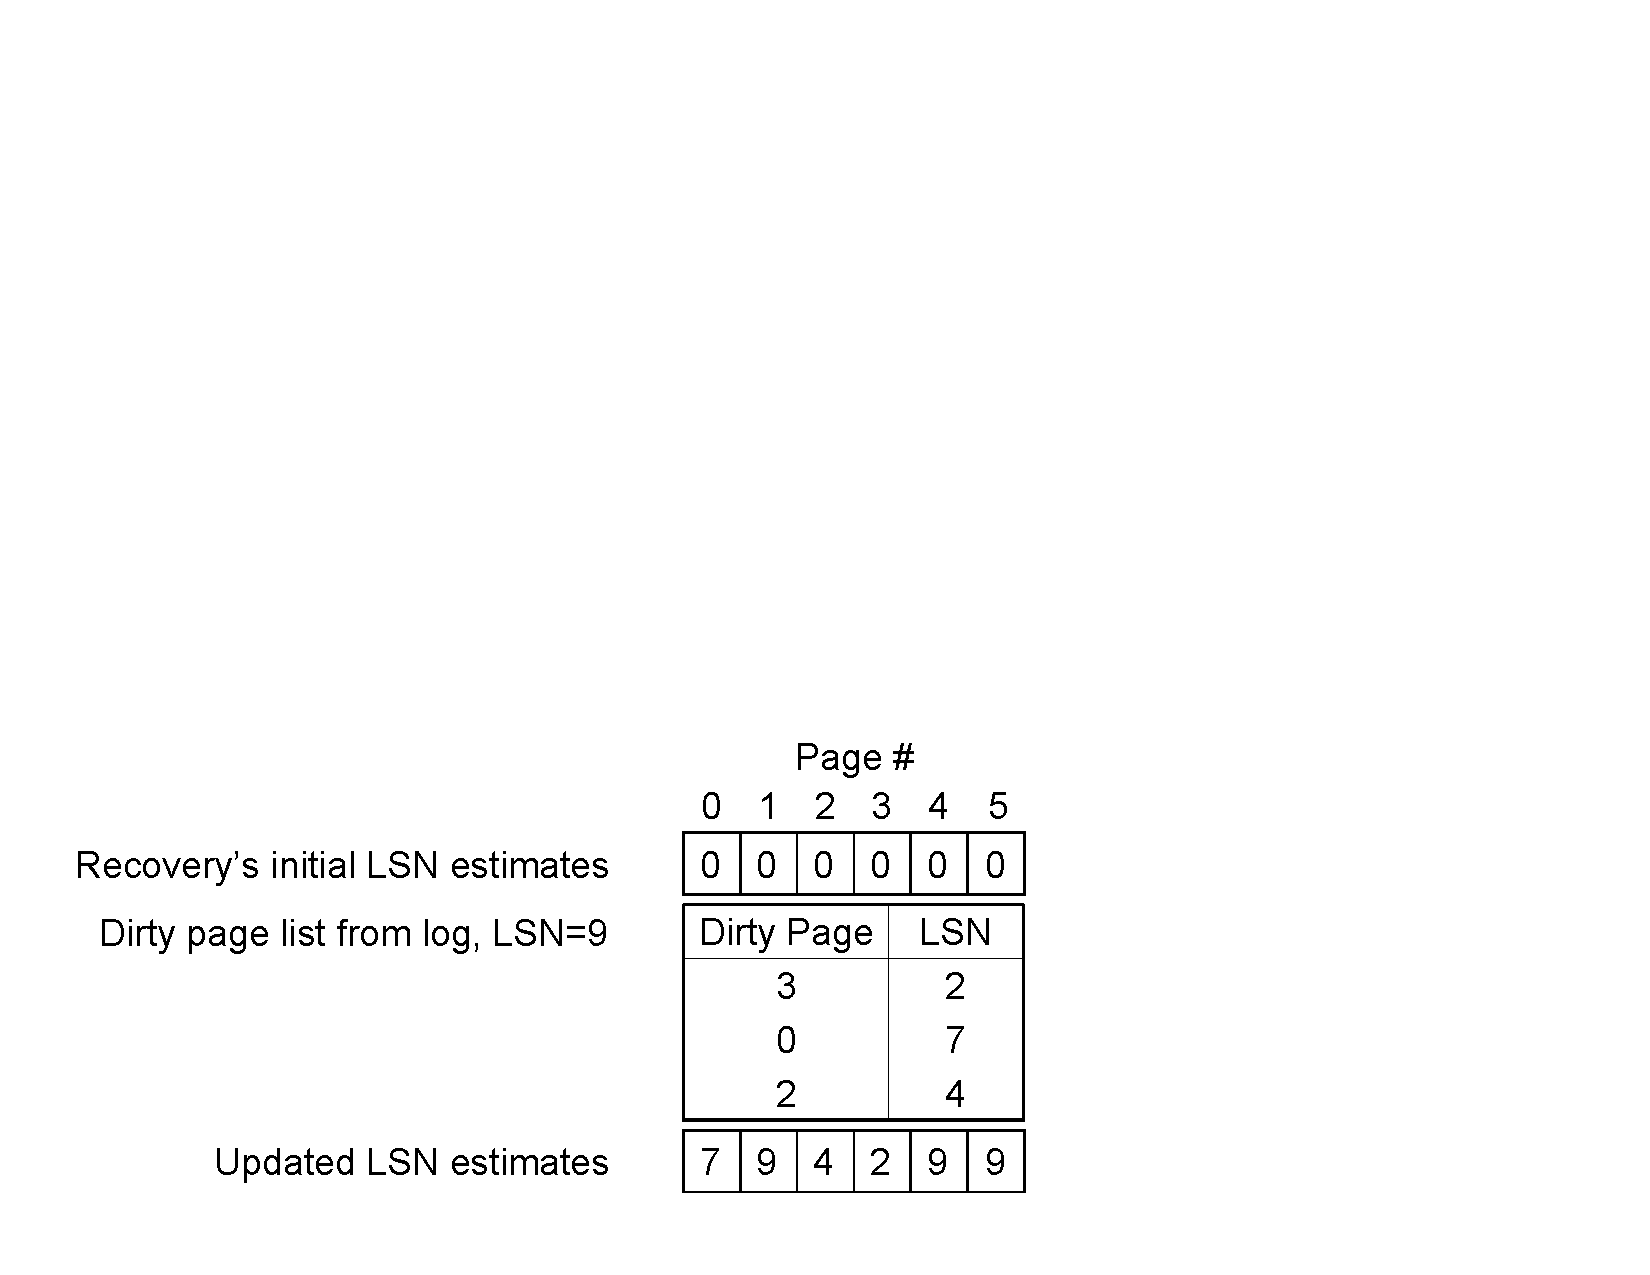
\includegraphics[%
  viewport=0bp 0bp 460bp 225bp,
  clip,
  width=1\columnwidth]{figs/lsn-estimation.pdf}
\caption{\label{fig:lsn-estimation}LSN estimation.  If a page is not mentioned in the checkpoint, it must be up to date on disk.}
\vspace{-12pt}
\end{figure}


Although the mechanism used for recovery is similar, the invariants
maintained during recovery have changed.  With conventional
transactions, if a page in the page file is internally consistent
immediately after a crash, then the page will remain internally
consistent throughout the recovery process.  This is not the case with
our LSN-free scheme.  Internal page inconsistencies may be introduced
because recovery has no way of knowing the exact version of a page.
Therefore, it may overwrite new portions of a page with older data
from the log.  The page will then contain a mixture of new and
old bytes, and any data structures stored on the page may be
inconsistent.  However, once the redo phase is complete, any old bytes
will be overwritten by their most recent values, so the page will
return to a self-consistent up-to-date state.
(Section~\ref{sec:torn-page} explains this in more detail.)

Undo is unaffected except that any redo records it produces must be
blind updates just like normal operation.  We don't expect this to be
a practical problem.

The rest of this section describes how concurrent, LSN-free pages 
allow standard file system and database optimizations to be easily
combined, and shows that the removal of LSNs from pages
simplifies recovery while increasing its flexibility.

\subsection{Zero-copy I/O} 

We originally developed LSN-free pages as an efficient method for
transactionally storing and updating multi-page objects, called {\em
blobs}.  If a large object is stored in pages that contain LSNs, then it is not contiguous on disk, and must be gathered together by using the CPU to do an expensive copy into a second buffer.

In contrast, modern file systems allow applications to
perform a DMA copy of the data into memory, allowing the CPU to be used for
more productive purposes.  Furthermore, modern operating systems allow
network services to use DMA and network adaptor hardware to read data
from disk, and send it over a network socket without passing it
through the CPU.  Again, this frees the CPU, allowing it to perform
other tasks.

We believe that LSN-free pages will allow reads to make use of such
optimizations in a straightforward fashion.  Zero-copy writes are
 more challenging, but the goal would be to use one sequential write
to put the new version on disk and then update meta data accordingly.
We need not put the blob in the log if we avoid update in place; most
blob implementations already avoid update in place since the length may vary between writes.  We suspect that contributions from log-based file
systems~\cite{lfs} can address these issues. In particular, we
imagine writing large blobs to a distinct log segment and just
entering metadata in the primary log.

%In
%the worst case, the blob would have to be relocated in order to
%defragment the storage.  Assuming the blob is relocated once, this
%would amount to a total of three, mostly sequential zero-copy disk operations.
%(Two writes and one read.)  However, in the best case, the blob would
%only be written once.  In contrast, conventional blob implementations
%generally write the blob twice, and use the CPU to copy the data onto pages.  \yad could also provide 
%file system semantics, and use DMA to update blobs in place.

\subsection{Concurrent RVM}

Our LSN-free pages are similar to the recovery scheme used by
recoverable virtual memory (RVM) and Camelot~\cite{camelot}. RVM
used purely physical logging and LSN-free pages so that it
could use {\tt mmap} to map portions of the page file into application
memory~\cite{lrvm}.  However, without support for logical log entries
and nested top actions, it is difficult to implement a
concurrent, durable data structure using RVM or Camelot.  (The description of
Argus in Section~\ref{sec:argus} sketches one
 approach.)

In contrast, LSN-free pages allow logical
undo and therefore nested top actions and concurrent
transactions; a concurrent data structure need only provide \yad
with an appropriate inverse each time its logical state changes.

We plan to add RVM-style transactional memory to \yad in a way that is
compatible with fully concurrent in-memory data structures such as
hash tables and trees, and with existing
\yad data structure implementations.


\subsection{Unbounded Atomicity}
\label{sec:torn-page}

%Recovery schemes that make use of per-page LSNs assume that each page
%is written to disk atomically even though that is generally no longer
%the case in modern disk drives.  Such schemes deal with this problem
%by using page formats that allow partially written pages to be
%detected.  Media recovery allows them to recover these pages.

Unlike transactions with per-page LSNs, transactions based on blind 
updates do not require atomic page writes
and thus impose no meaningful boundaries on atomic updates.  We still
use pages to simplify integration into the rest of the system, but
need not worry about torn pages.  In fact, the redo phase of the
LSN-free recovery algorithm effectively creates a torn page each time it
applies an old log entry to a new page.  However, it guarantees that
all such torn pages will be repaired by the time redo completes.  In
the process, it also repairs any pages that were torn by a crash.
This also implies that blind-update transactions work with storage technologies with
different (and varying or unknown) units of atomicity.

Instead of relying upon atomic page updates, LSN-free recovery relies
on a weaker property, which is that each bit in the page file must
be either:
\begin{enumerate}
\item The version that was being overwritten at the crash.
\item The newest version of the bit written to storage.
\item Detectably corrupt (the storage hardware issues an error when the
  bit is read).
\end{enumerate}

Modern drives provide these properties at a sector level: Each sector
is updated atomically, or it fails a checksum when read, triggering an
error.  If a sector is found to be corrupt, then media recovery can be
used to restore the sector from the most recent backup.

To ensure that we correctly update all of the old bits, we simply
play the log forward from a point in time that is known to be older than the
LSN of the page (which we must estimate).  For bits that are
overwritten, we end up with the correct version, since we apply the
updates in order.  For bits that are not overwritten, they must have
been correct before and remain correct after recovery.  Since all
operations performed by redo are blind updates, they can be applied
regardless of whether the initial page was the correct version or even
logically consistent.

\begin{figure}
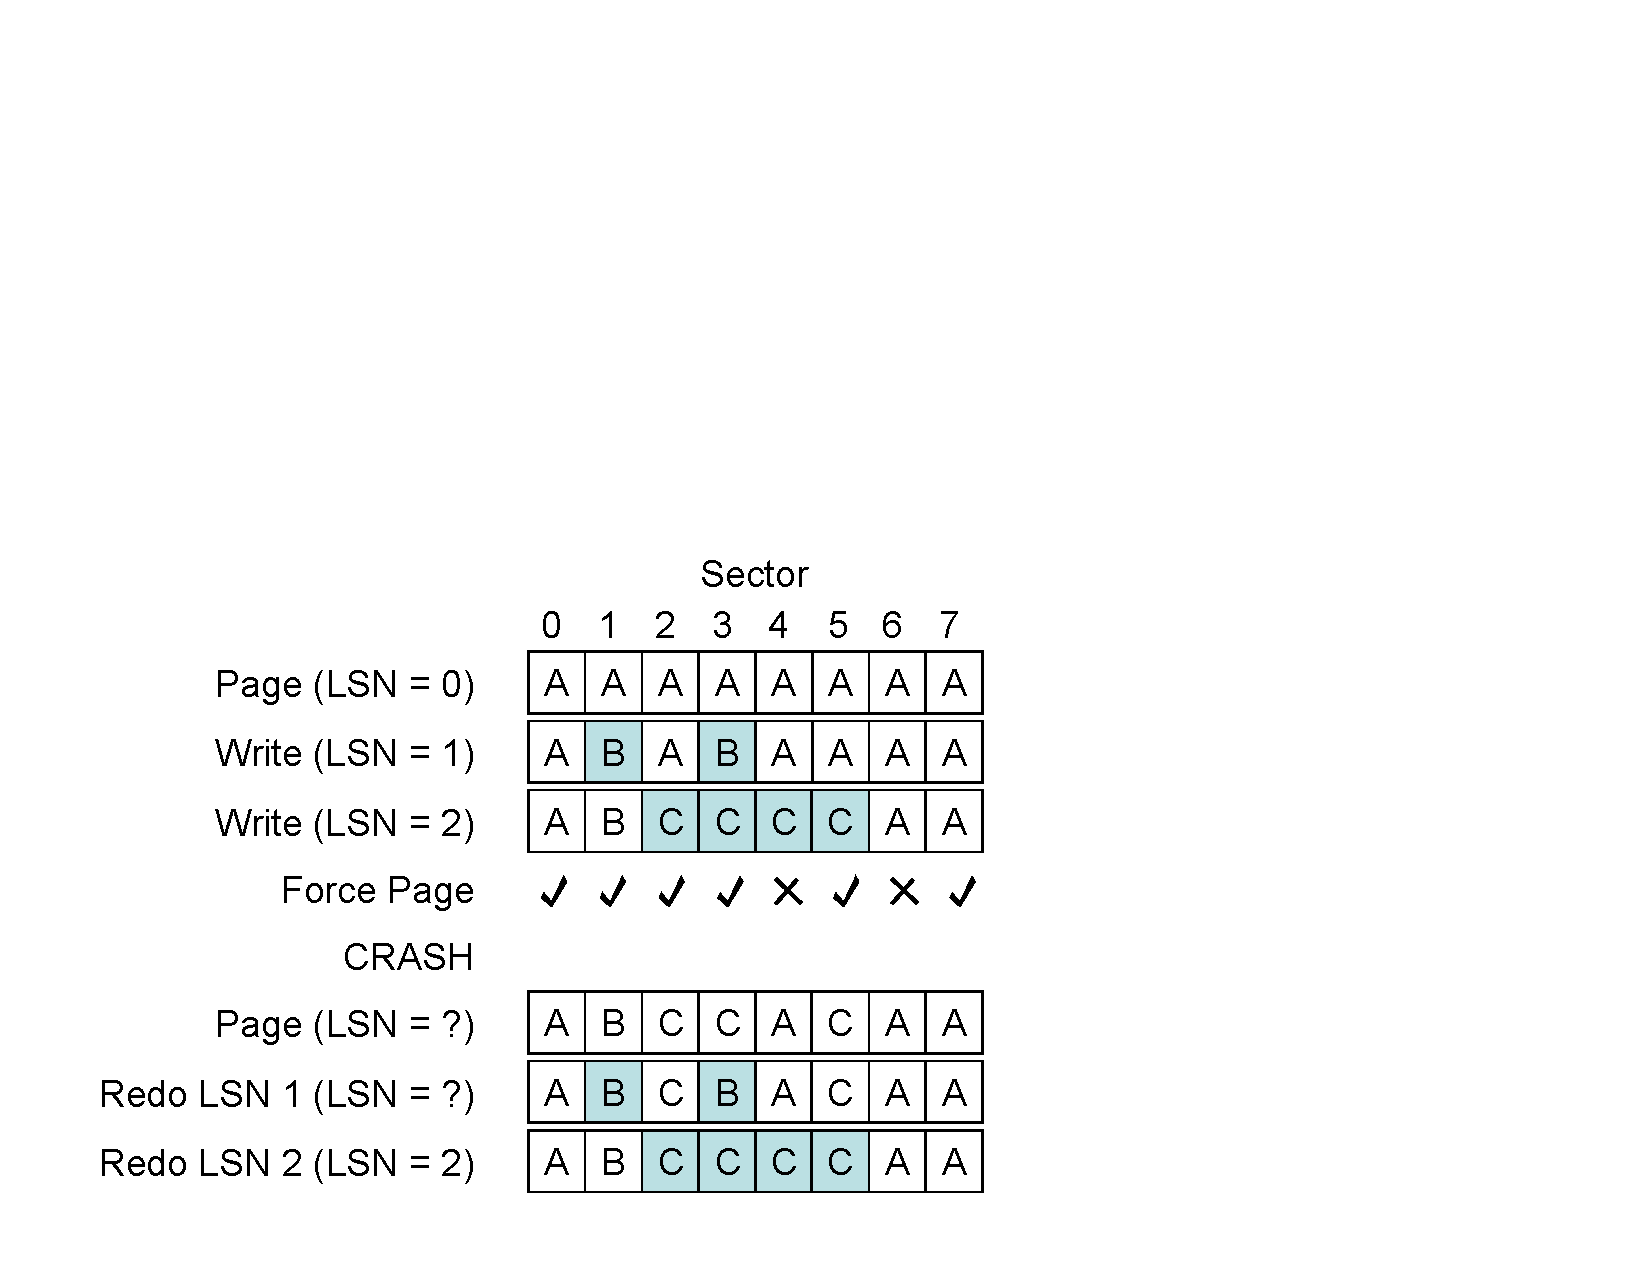
\includegraphics[%
  viewport=0bp 0bp 445bp 308bp,
  clip,
  width=1\columnwidth]{figs/torn-page.pdf}
\caption{\label{fig:torn}Torn pages and LSN-free recovery.
The page is torn during the crash, but consistent once redo completes.
Overwritten sectors are shaded.}
\vspace{-12pt}
\end{figure}

Figure~\ref{fig:torn} describes a page that is torn during crash, and the actions performed by redo that repair it.  Assume that the initial version
of the page, with LSN $0$, is on disk, and the disk is in the process
of writing out the version with LSN $2$ when the system crashes.  When
recovery reads the page from disk, it may encounter any combination of
sectors from these two versions.

Note that sectors zero, six and seven are not overwritten by any of
the log entries that Redo will play back.  Therefore, their values are
unchanged in both versions of the page.  In the example, zero and seven 
are overwritten during the crash, while six is left
over from the old version of the page.

Redoing LSN 1 is unnecessary, since all of its sectors happened to
make it to disk.  However, recovery has no way of knowing this and
applies the entry to the page, replacing sector three with an older 
version.  When LSN 2 is applied, it brings this sector up to date,
and also overwrites sector four, which did not make it to
disk.  At this point, the page is internally consistent.

Since LSN-free recovery only relies upon atomic updates at the bit
level, it decouples page boundaries from atomicity and recovery.  This
allows operations to manipulate atomically (potentially
non-contiguous) regions of arbitrary size by producing a single log
entry.  If this log entry includes a logical undo function (rather
than a physical undo), then it can serve the purpose of a nested top
action without incurring the extra log bandwidth of storing physical
undo information.  Such optimizations can be implemented using
conventional transactions, but they appear to be easier to implement
and reason about when applied to LSN-free pages.

\subsection{Summary}

In these last two sections, we explored some of the flexibility of \yad. This
includes user-defined operations, combinations of steal and force on
a per-operation basis, flexible locking options, and a new class of
transactions based on blind updates that enables better support for
DMA, large objects, and multi-page operations.  In the next section,
we show through experiments how this flexibility enables important
optimizations and a wide-range of transactional systems.




\section{Experiments}
\label{experiments}

\yad provides applications with the ability to customize storage
routines and recovery semantics.  In this section, we show that this
flexibility does not come with a significant performance cost for
general-purpose transactional primitives, and show how a number of
special-purpose interfaces aid in the development of higher-level 
code while significantly improving application performance.

\subsection{Experimental setup}
\label{sec:experimental_setup}

We chose Berkeley DB in the following experiments because
it provides transactional storage primitives
similar to \yad, is 
commercially maintained and is designed for high performance and high
concurrency.  For all tests, the two libraries provide the same
transactional semantics unless explicitly noted.

All benchmarks were run on an Intel Xeon 2.8 GHz processor with 1GB of RAM and a
10K RPM SCSI drive using ReiserFS~\cite{reiserfs}.\endnote{We found that the
  relative performance of Berkeley DB and \yad under single-threaded testing is sensitive to
  file system choice, and we plan to investigate the reasons why the
  performance of \yad under ext3 is degraded. However, the results
  relating to the \yad optimizations are consistent across file system
  types.}  All results correspond to the mean of multiple runs with a
95\% confidence interval with a half-width of 5\%.

We used Berkeley DB 4.2.52 
%as it existed in Debian Linux's testing branch during March of 2005, 
with the flags DB\_TXN\_SYNC (sync log on commit), and
DB\_THREAD (thread safety) enabled.  We 
increased Berkeley DB's buffer cache and log buffer sizes to match
\yads default sizes.  If
Berkeley DB implements a feature that \yad is missing we enable it if it 
improves performance.  

We disable Berkeley DB's lock manager for the benchmarks,
though we use ``Free Threaded'' handles for all
tests.  This significantly increases performance by
eliminating transaction deadlock, abort, and
repetition.  However, disabling the lock manager caused 
concurrent Berkeley DB benchmarks to become unstable, suggesting either a
bug or misuse of the feature.  
With the lock manager enabled, Berkeley
DB's performance in the multi-threaded benchmark (Section~\ref{sec:lht}) strictly decreased with
increased concurrency.  

We expended a considerable effort tuning Berkeley DB and our efforts
significantly improved Berkeley DB's performance on these tests.
Although further tuning by Berkeley DB experts would probably improve
Berkeley DB's numbers, we think our comparison shows that the systems'
performance is comparable.  As we add functionality, optimizations,
and rewrite modules, \yads relative performance varies.  We expect
\yads extensions and custom recovery mechanisms to continue to
perform similarly to comparable monolithic implementations.

\subsection{Linear hash table}
\label{sec:lht}

\begin{figure}[t]
\graphdbg{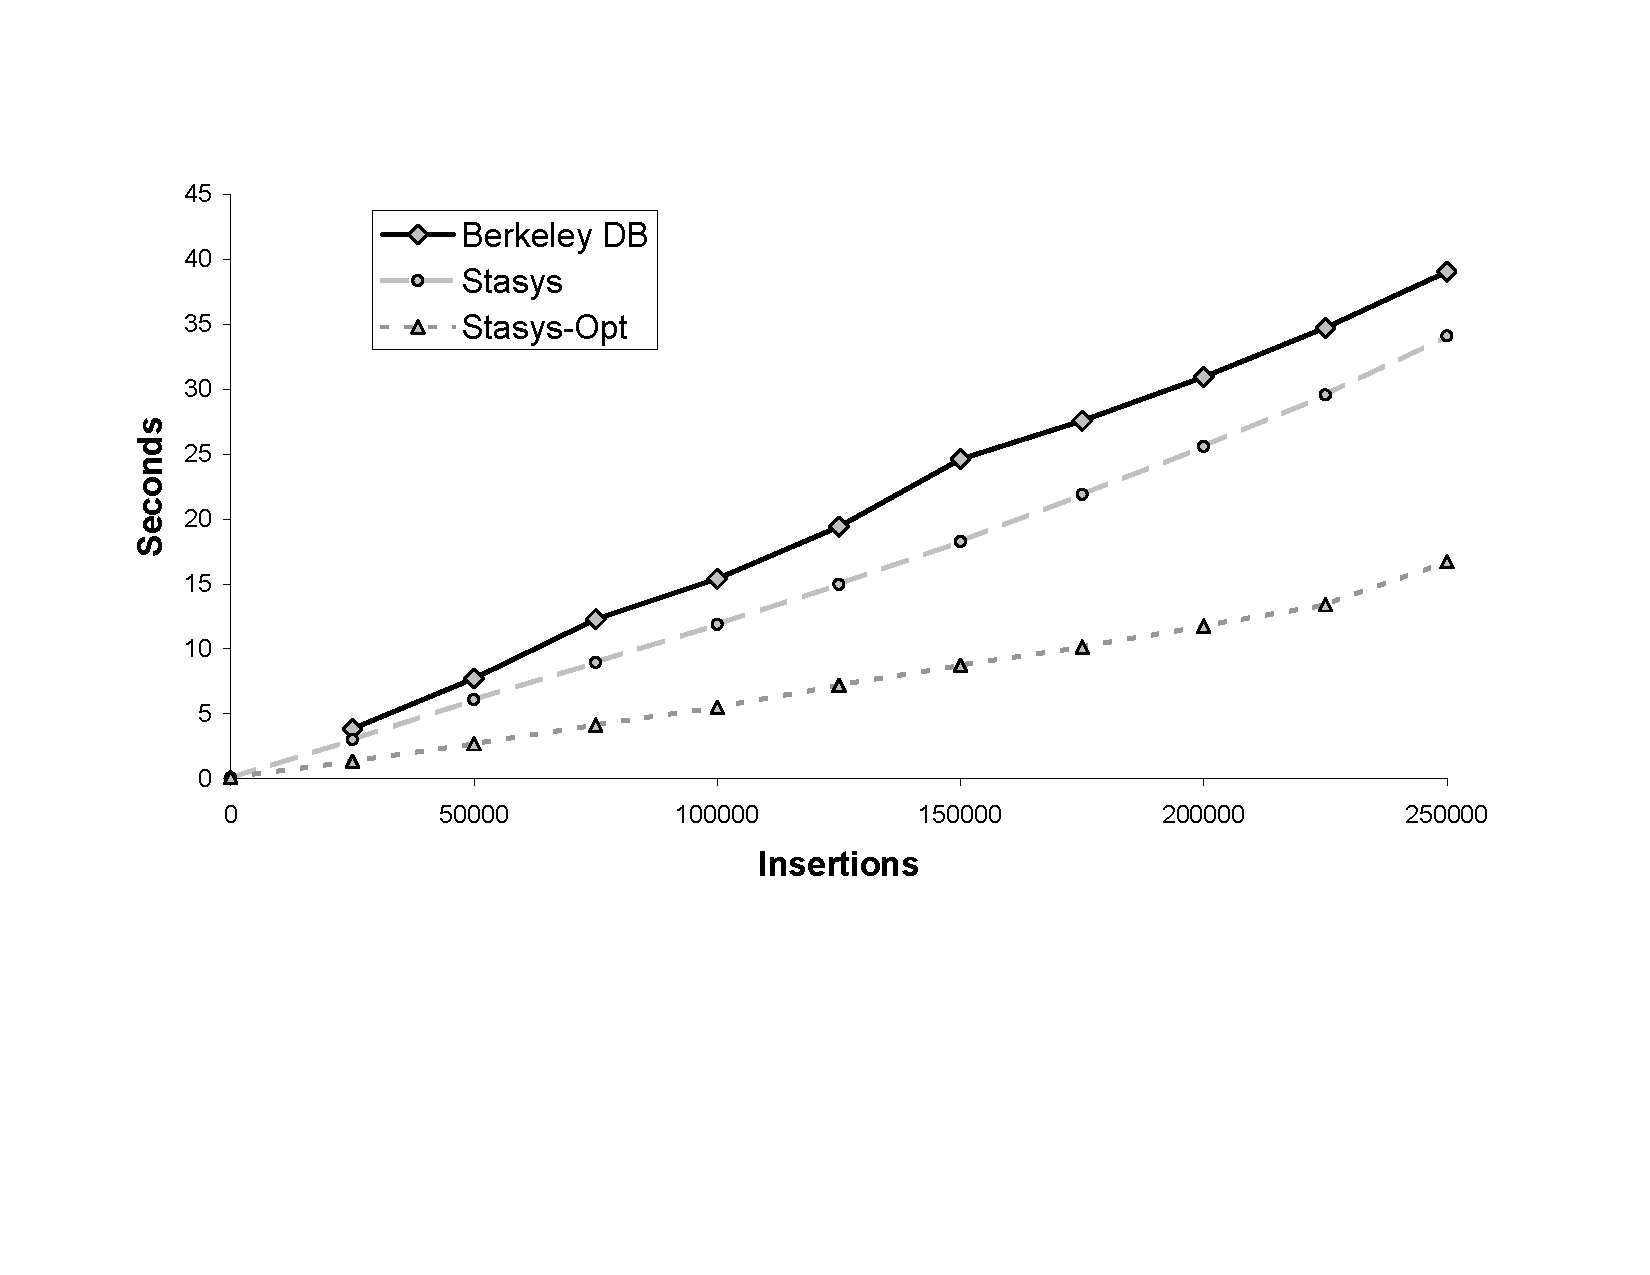
\includegraphics[%
    viewport=-23bp 28bp 625bp 360bp, 
    clip,
   width=1\columnwidth]{figs/bulk-load.pdf}}
%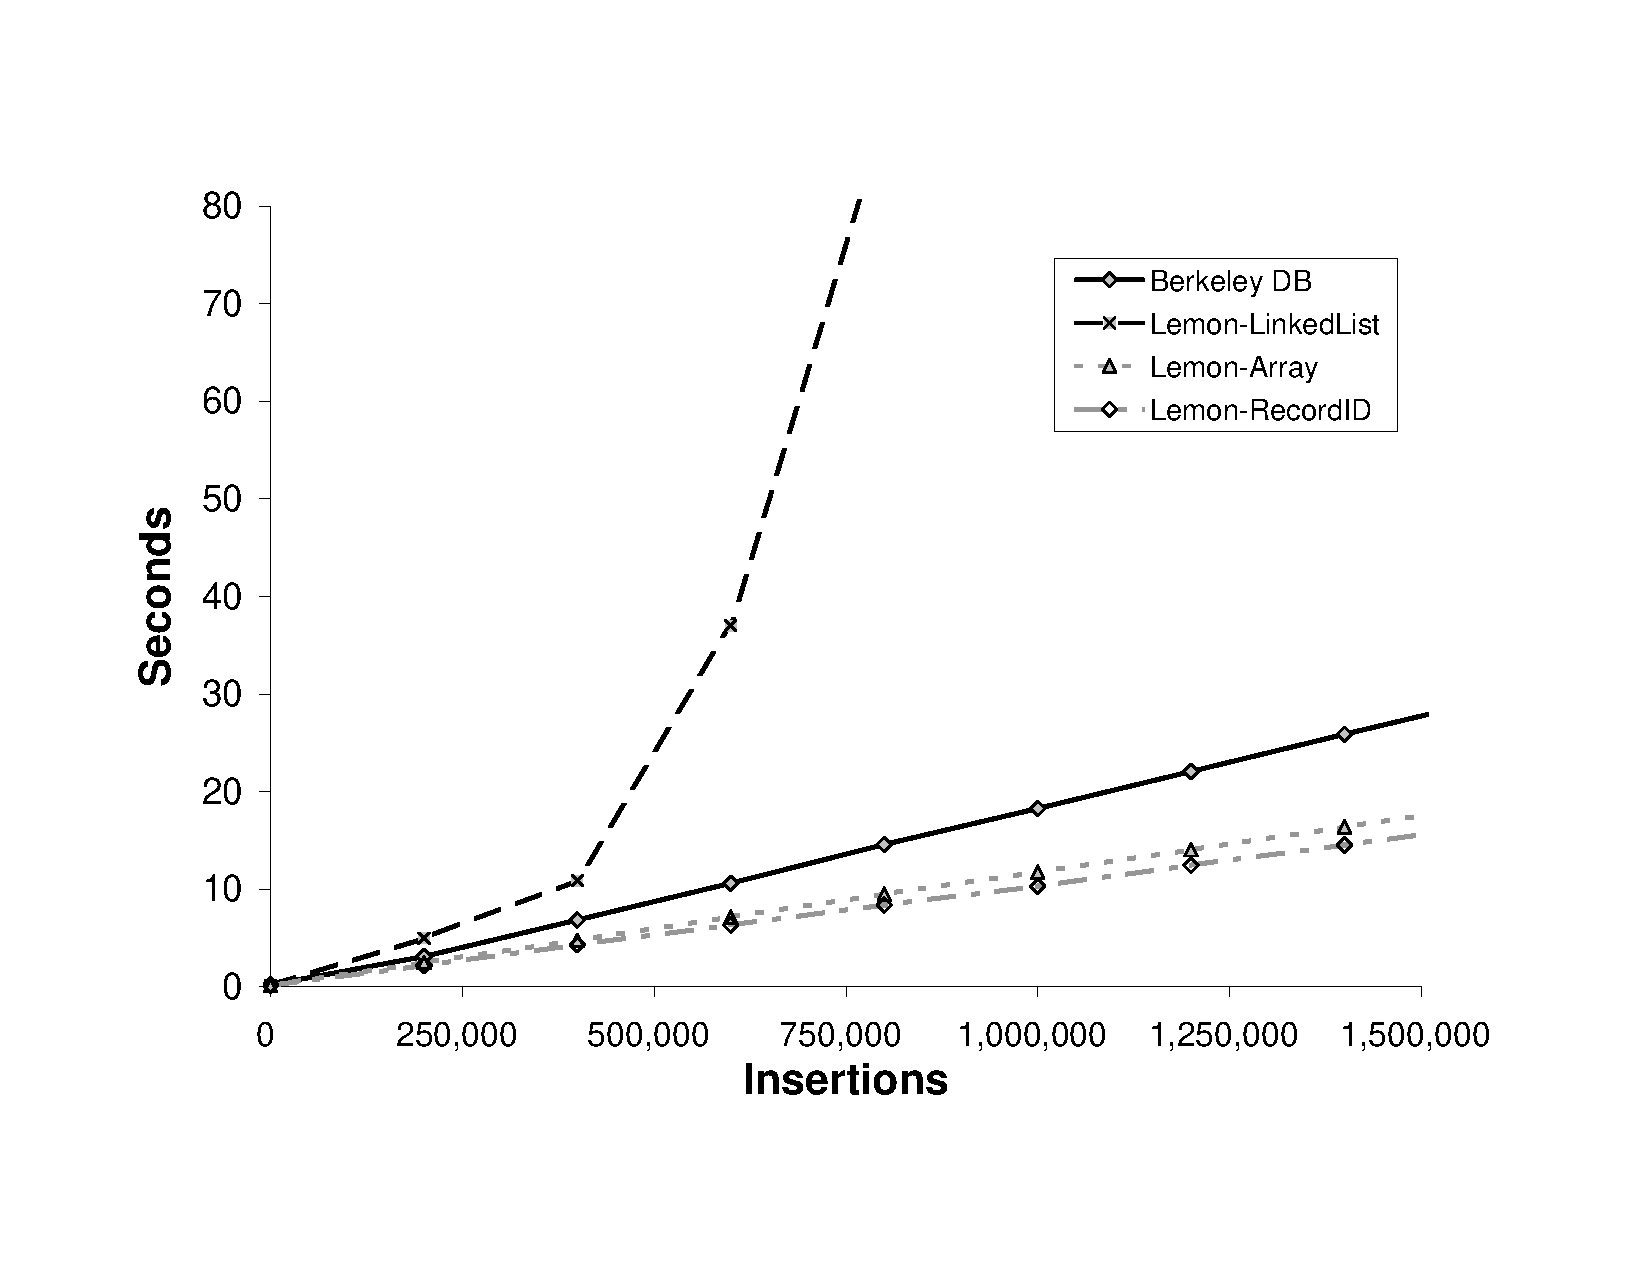
\includegraphics[%
%   width=1\columnwidth]{bulk-load-raw.pdf}1
\caption{\label{fig:BULK_LOAD} Performance of \yad and Berkeley DB hash table implementations.  The
test is run as a single transaction, minimizing overheads due to synchronous log writes.}
\end{figure}

\begin{figure}[t]
%\hspace*{18pt}
%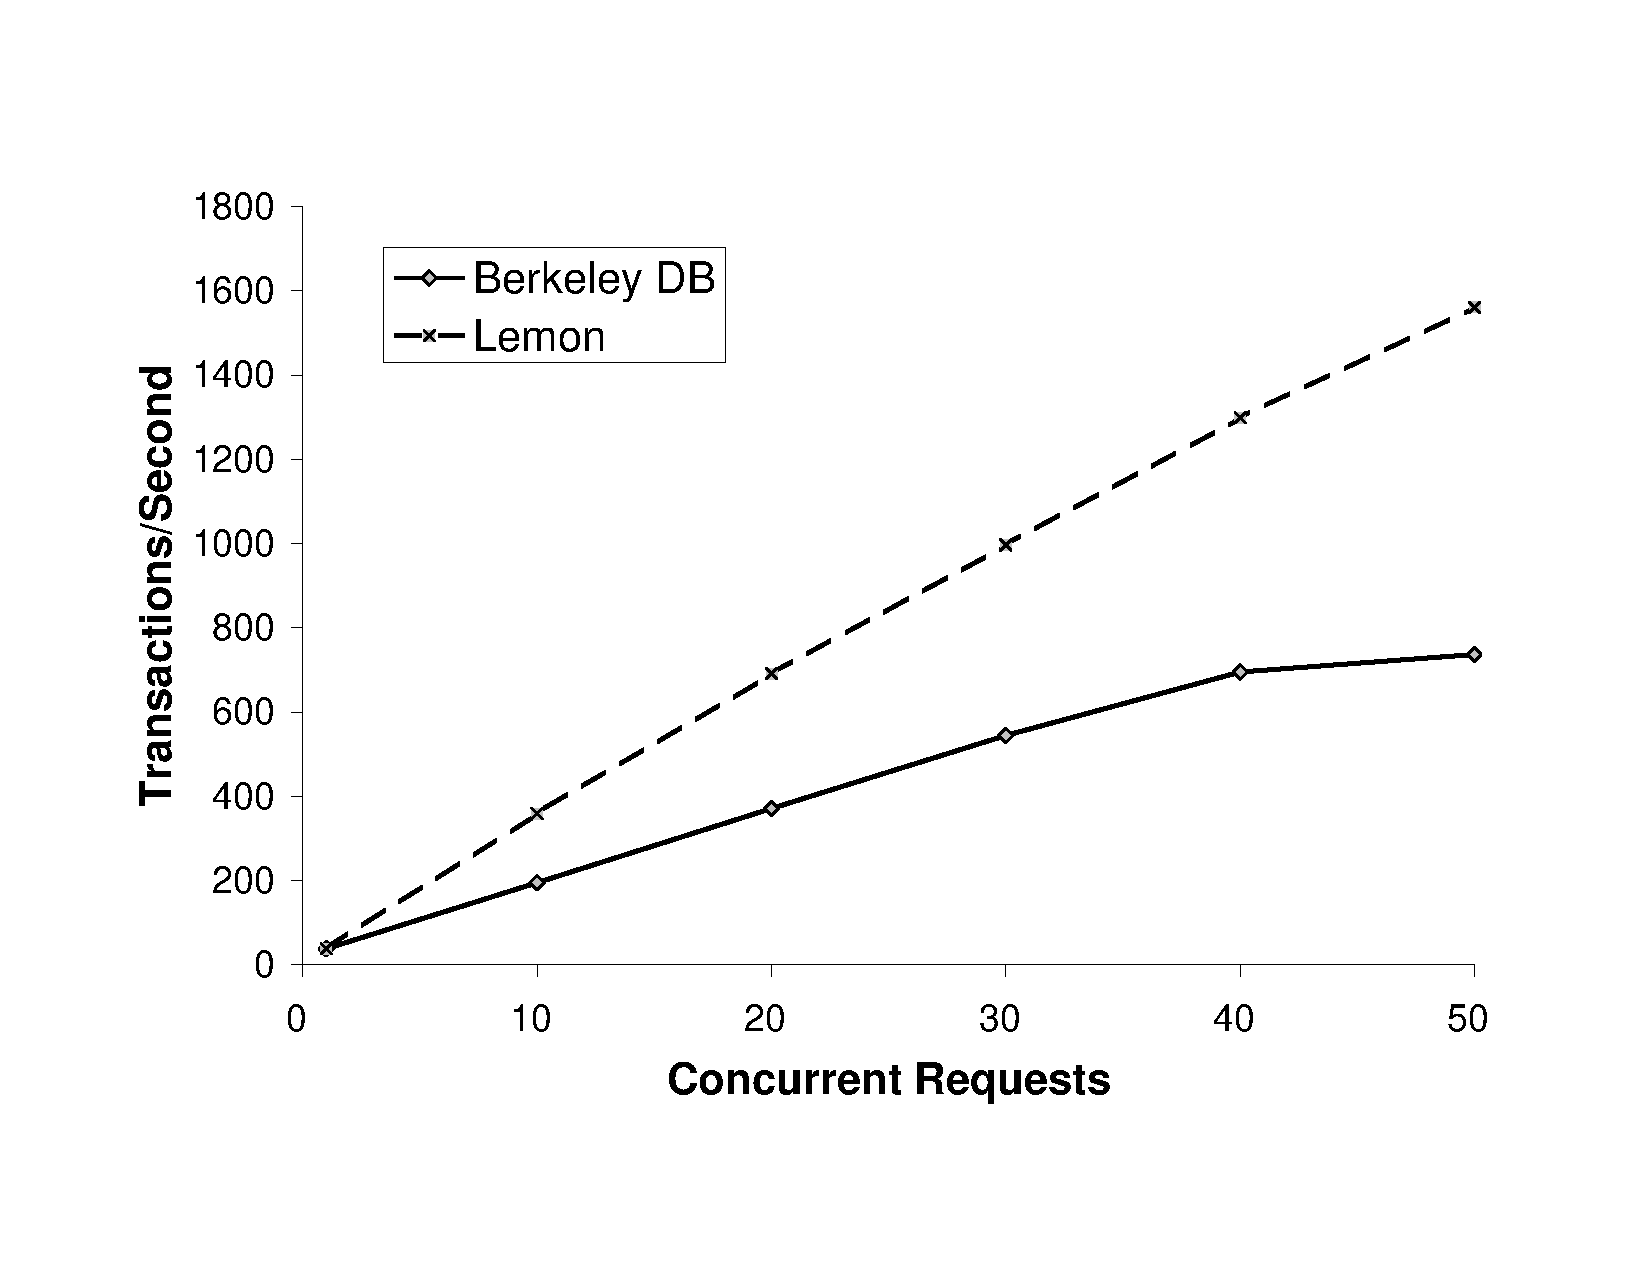
\includegraphics[%
%   width=1\columnwidth]{tps-new.pdf}
\graphdbg{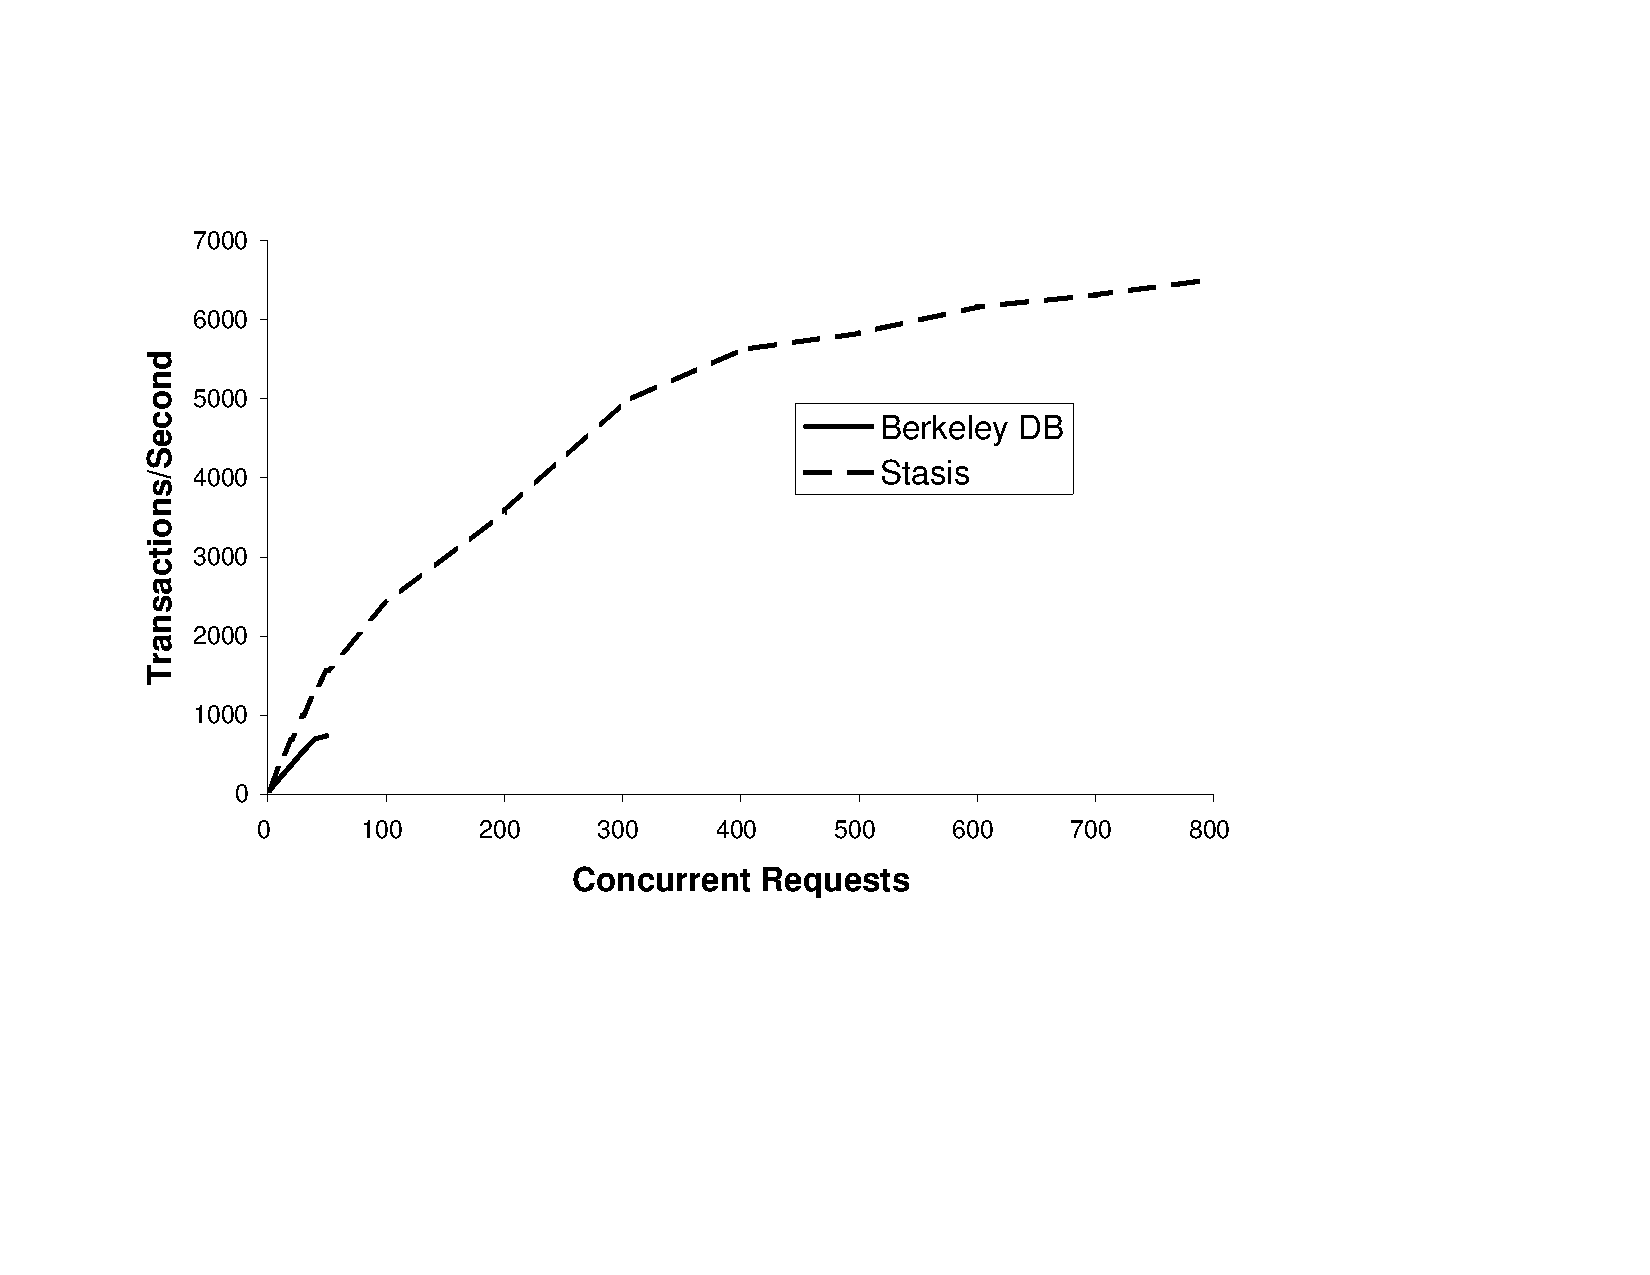
\includegraphics[%
    viewport=-43bp 50bp 490bp 370bp, 
    clip,
   width=1\columnwidth]{figs/tps-extended.pdf}}
\caption{\label{fig:TPS} High concurrency hash table performance of Berkeley DB and \yad.  We were unable to get Berkeley DB to work correctly with more than 50 threads (see text).
\vspace{-12pt}
}
\end{figure}

This section presents two hash table implementations built on top of
\yad, and compares them with the hash table provided by Berkeley DB.
One of the \yad implementations is simple and modular, while
the other is monolithic and hand-tuned.  Our experiments show that
\yads performance is competitive, both with single-threaded and
high-concurrency transactions.

%Although the beginning of this paper describes the limitations of
%physical database models and relational storage systems in great
%detail, these systems are the basis of most common transactional
%storage routines.  Therefore, we implement a key-based access method
%in this section. We argue that obtaining reasonable performance in
%such a system under \yad is straightforward.  We then compare our
%straightforward, modular implementation to our hand-tuned version and
%Berkeley DB's implementation.

The modular hash table uses nested top actions to update its internal
structure atomically.  It uses a {\em linear} hash
function~\cite{lht}, allowing it to increase capacity incrementally.
It is based on a number of modular subcomponents.  Notably, the
physical location of each bucket is stored in a growable array of
fixed-length entries.  The bucket lists can be provided by either of
\yads linked list implementations.  One provides fixed-length entries,
yielding a hash table with fixed-length keys and values.  The list
(and therefore hash table) used in our experiments provides variable-length entries.

The hand-tuned hash table is also built on \yad and also uses a linear hash
function.  However, it is monolithic and uses carefully ordered writes to
reduce runtime overheads such as log bandwidth.  Berkeley DB's
hash table is a popular, commonly deployed implementation, and serves
as a baseline for our experiments.

Both of our hash tables outperform Berkeley DB on a workload that bulk
loads the tables by repeatedly inserting $(key, value)$ pairs
(Figure~\ref{fig:BULK_LOAD}).
%although we do not wish to imply this is always the case.
%We do not claim that our partial implementation of \yad
%generally outperforms, or is a robust alternative
%to Berkeley DB.  Instead, this test shows that \yad is comparable to
%existing systems, and that its modular design does not introduce gross
%inefficiencies at runtime.
The performance of the modular hash table shows that
data structure implementations composed from
simpler structures can perform comparably to the implementations included 
in existing monolithic systems.  The hand-tuned
implementation shows that \yad allows application developers to
optimize important primitives.

% I cut this because Berkeley db supports custom data structures....

%In the
%best case, past systems allowed application developers to provide
%hints to improve performance.  In the worst case, a developer would be
%forced to redesign and application to avoid sub-optimal properties of
%the transactional data structure implementation.

Figure~\ref{fig:TPS} describes the performance of the two systems under
highly concurrent workloads using the ext3 file system.\endnote{Multi-threaded benchmarks
  were performed using an ext3 file system. 
  Concurrency caused both Berkeley DB and \yad to behave unpredictably
  under ReiserFS was used.  \yads multi-threaded throughput
  was significantly better than Berkeley DB's with both file systems.}
  For this test, we used the modular
hash table, since we are interested in the performance of a 
simple, clean data structure implementation that a typical system implementor might
produce, not the performance of our own highly tuned implementation.

Both Berkeley DB and \yad can service concurrent calls to commit with
a single synchronous I/O.
\yad scaled quite well, delivering over 6000 transactions per
second,\endnote{The concurrency test was run without lock managers, and the
  transactions obeyed the A, C, and D properties.  Since each
  transaction performed exactly one hash table write and no reads, they also
  obeyed I (isolation) in a trivial sense.}  and provided roughly
double Berkeley DB's throughput (up to 50 threads).  Although not
shown here, we found that the latencies of Berkeley DB and \yad were
similar.


\begin{figure*}
\graphdbg{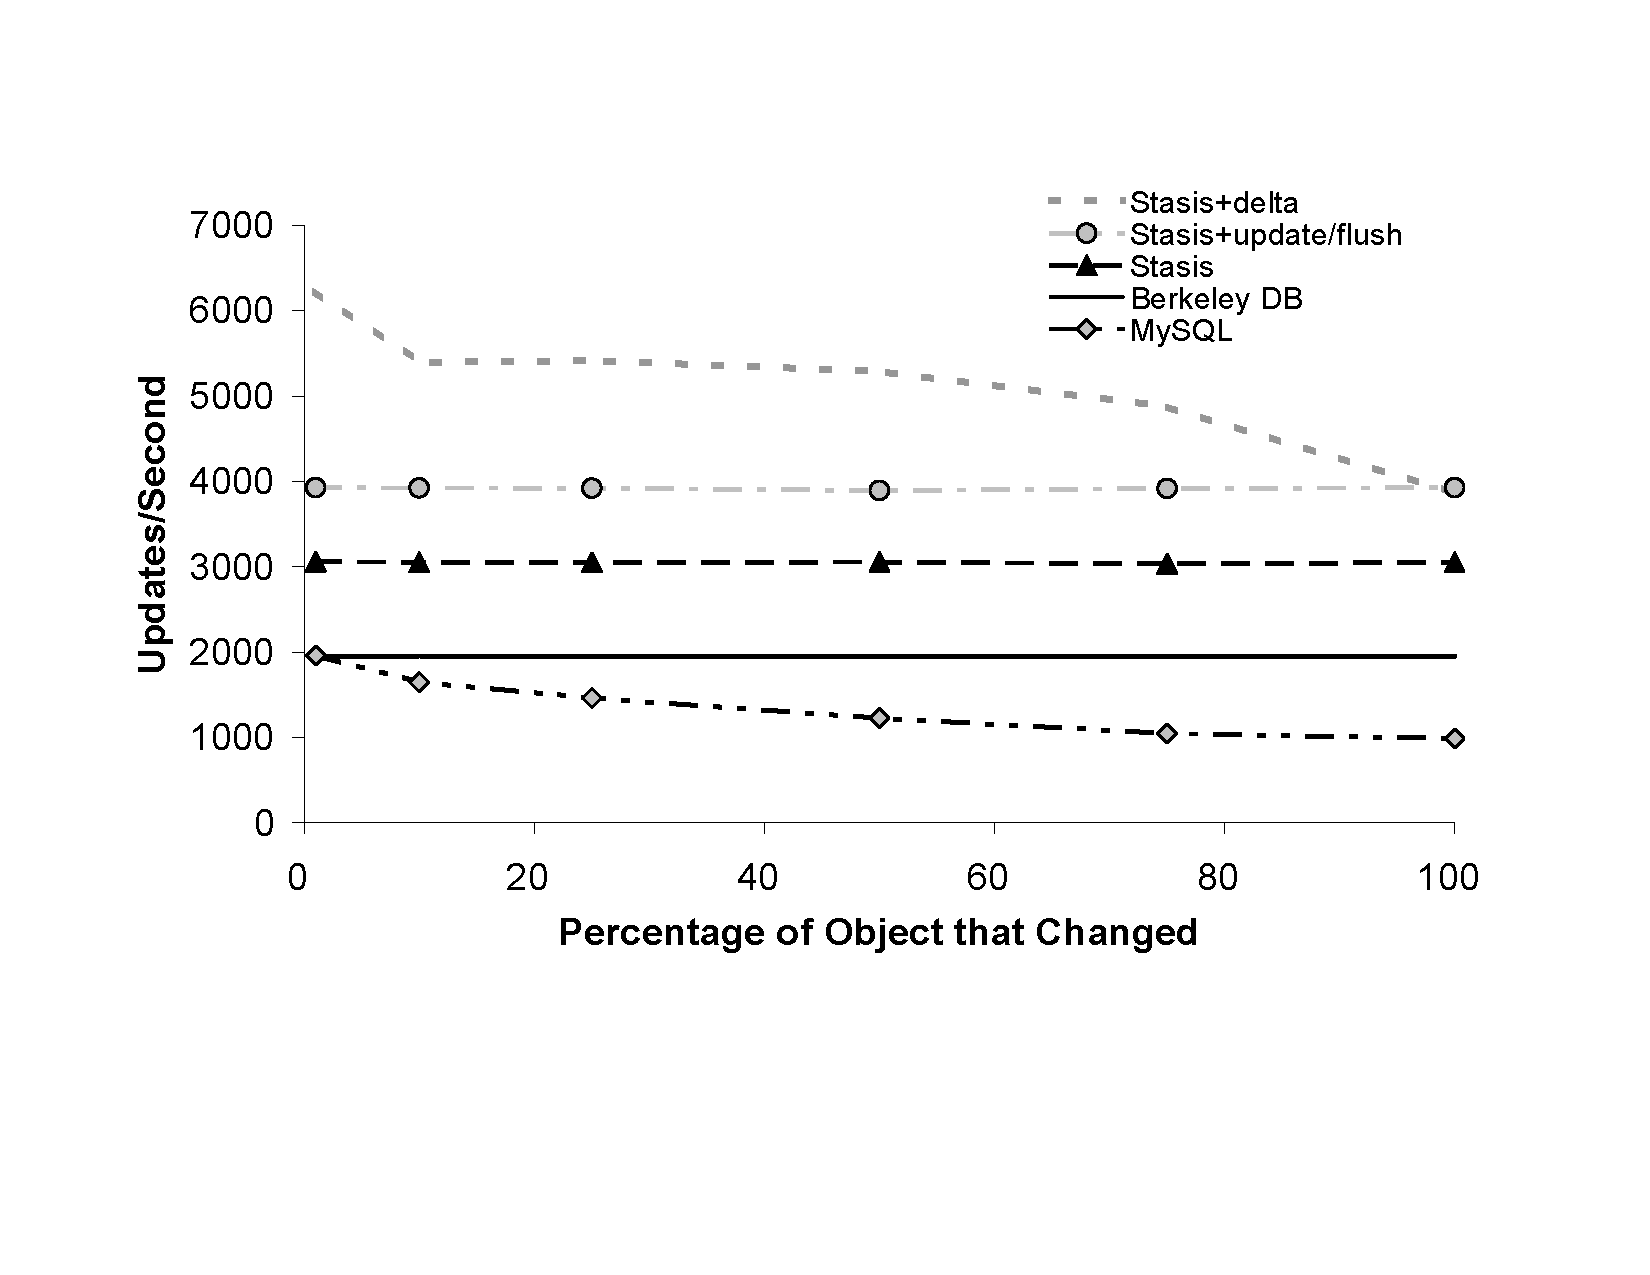
\includegraphics[%
    viewport=-15bp 19bp 650bp 400bp, 
    clip,
    width=1\columnwidth]{figs/object-diff.pdf}}
\hspace{.2in}
\graphdbg{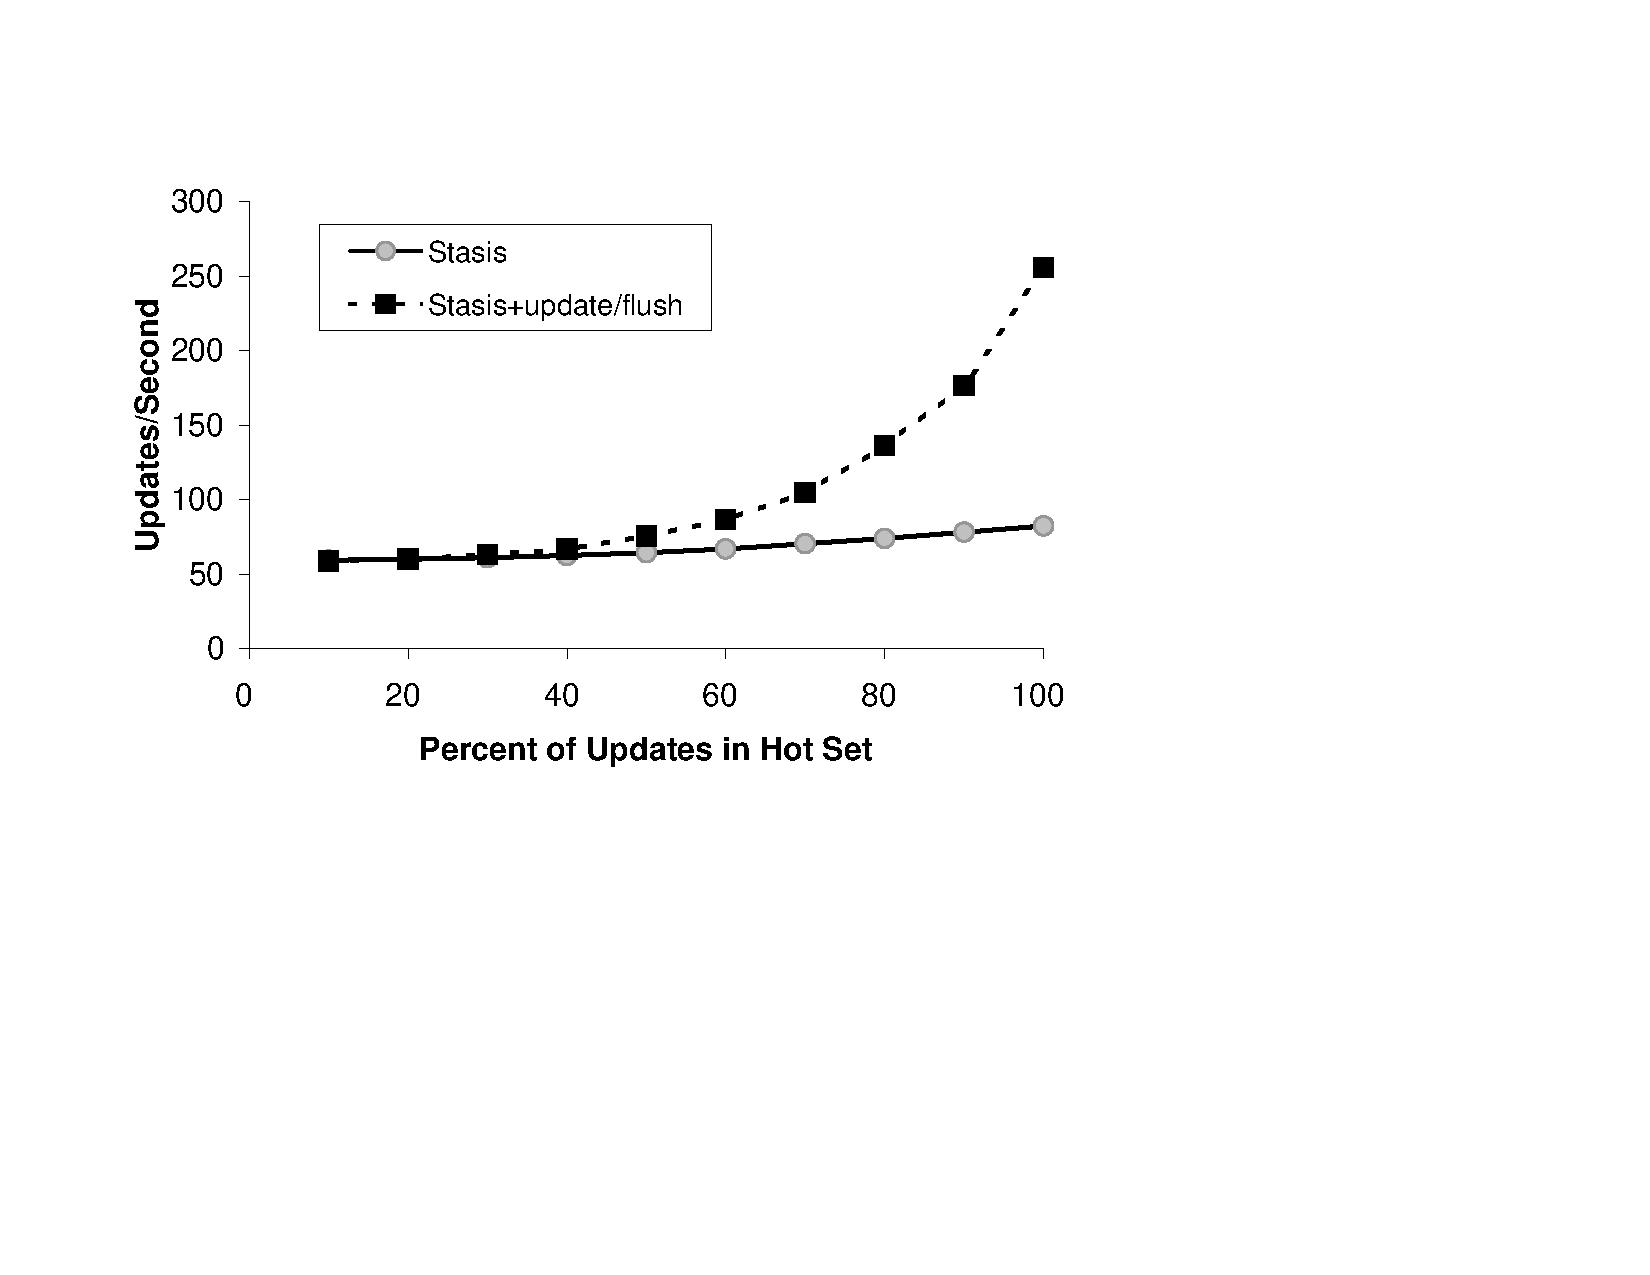
\includegraphics[%
%    viewport=-25bp 23bp 425bp 330bp, 
    viewport=-50bp 28bp 460bp 315bp, 
    clip,
    width=1\columnwidth]{figs/mem-pressure.pdf}}
\caption{\label{fig:OASYS}
The effect of \yad object persistence optimizations under low and high memory pressure.}
\vspace{-12pt}
\end{figure*}


\subsection{Object persistence}
\label{sec:oasys}

Two different styles of object persistence have been implemented
on top of \yad.
%\yad.  We could have just as easily implemented a persistence
%mechanism for a statically typed functional programming language, a
%dynamically typed scripting language, or a particular application,
%such as an email server.  In each case, \yads lack of a hard-coded data
%model would allow us to choose the representation and transactional
%semantics that make the most sense for the system at hand.
%
The first object persistence mechanism, pobj, provides transactional updates to objects in
Titanium, a Java variant.  It transparently loads and persists
entire graphs of objects, but will not be discussed in further detail.
The second variant was built on top of a C++ object
persistence library, \oasys.  \oasys uses plug-in storage
modules that implement persistent storage, and includes plugins
for Berkeley DB and MySQL.  

This section describes how the \yad plugin supports optimizations that reduce the
amount of data written to log and halve the amount of RAM required.
We present three variants of the \yad plugin.  The basic one treats
\yad like Berkeley DB.  The ``update/flush'' variant
customizes the behavior of the buffer manager. Finally, the 
``delta'' variant uses update/flush, but only logs the differences
between versions.

The update/flush variant allows the buffer manager's view of live
application objects to become stale.  This is safe since the system is
always able to reconstruct the appropriate page entry from the live
copy of the object.  This reduces the number of times the
plugin must update serialized objects in the buffer manager, and
allows us to decrease drastically the amount of memory used by the
buffer manager.  

We implemented the \yad buffer pool optimization by adding two new
operations, update(), which updates the log when objects are modified, and flush(), which
updates the page when an object is evicted from the application's cache.  

The reason it would be difficult to do this with Berkeley DB is that
we still need to generate log entries as the object is being updated.
  This would cause Berkeley DB to write data to pages,
increasing the working set of the program and the amount of disk activity.

Furthermore, \yads copy of the objects is updated in the order objects
are evicted from cache, not the update order.
Therefore, the version of each object on a page cannot be determined
from a single LSN.

We solve this problem by using blind updates to modify
objects in place, but maintain a per-page LSN that is updated whenever
an object is allocated or deallocated.  At recovery, we apply
allocations and deallocations based on the page LSN.  To redo an
update, we first decide whether the object that is being updated
exists on the page.  If so, we apply the blind update.  If not, then
the object must have been freed, so we do not apply the
update. Because support for blind updates is only partially implemented, the
experiments presented below mimic this behavior at runtime, but do not
support recovery.

We also considered storing multiple LSNs per page and registering a
callback with recovery to process the LSNs.  However, in such a
scheme, the object allocation routine would need to track objects that
were deleted but still may be manipulated during redo.  Otherwise, it
could inadvertently overwrite per-object LSNs that would be needed
during recovery.
%
%\eab{we should at least implement this callback if we have not already}
%
Alternatively, we could arrange for the object pool 
to update atomically the buffer 
manager's copy of all objects that share a given page.

The third plugin variant, ``delta'', incorporates the update/flush
optimizations, but only writes changed portions of
objects to the log.  With \yads support for custom log
formats, this optimization is straightforward.

\oasys does not provide a transactional interface.
Instead, it is designed to be used in systems that stream objects over
an unreliable network connection.  The objects are independent of each
other, so each update should be applied atomically.  Therefore, there is
never any reason to roll back an applied object update.  Furthermore,
\oasys provides a sync method, which guarantees the durability of
updates after it returns.  In order to match these semantics as
closely as possible, \yads update/flush and delta optimizations do not
write any undo information to the log.  The \oasys sync method is
implemented by committing the current \yad transaction, and beginning
a new one.

As far as we can tell, MySQL and Berkeley DB do not support this
optimization in a straightforward fashion.  ``Auto-commit'' comes
close, but does not quite provide the same durability semantics as
\oasys' explicit syncs.

The operations required for the update/flush and delta optimizations required 
150 lines of C code, including whitespace, comments and boilerplate
function registrations.\endnote{These figures do not include the
  simple LSN-free object logic required for recovery, as \yad does not
  yet support LSN-free operations.}  Although the reasoning required
to ensure the correctness of this optimization is complex, the simplicity of
the implementation is encouraging.

In this experiment, Berkeley DB was configured as described above.  We
ran MySQL using InnoDB for the table engine.  For this benchmark, it
is the fastest engine that provides similar durability to \yad. We
linked the benchmark's executable to the {\tt libmysqld} daemon library,
bypassing the IPC layer. Experiments that used IPC were orders of magnitude slower.

Figure~\ref{fig:OASYS} presents the performance of the three \yad
variants, and the \oasys plugins implemented on top of other
systems.  In this test, none of the systems were memory bound.  As
we can see, \yad performs better than the baseline systems, which is
not surprising, since it is not providing the A property of ACID
transactions.

In non-memory bound systems, the optimizations nearly double \yads
performance by reducing the CPU overhead of marshalling and
unmarshalling objects, and by reducing the size of log entries written
to disk.

To determine the effect of the optimization in memory bound systems,
we decreased \yads page cache size, and used O\_DIRECT to bypass the
operating system's disk cache.  We partitioned the set of objects
so that 10\% fit in a {\em hot set}.
Figure~\ref{fig:OASYS} also presents \yads performance as we varied the
percentage of object updates that manipulate the hot set.  In the
memory bound test, we see that update/flush indeed improves memory
utilization.

\subsection{Request reordering}


\label{sec:logging}
\begin{figure}
\graphdbg{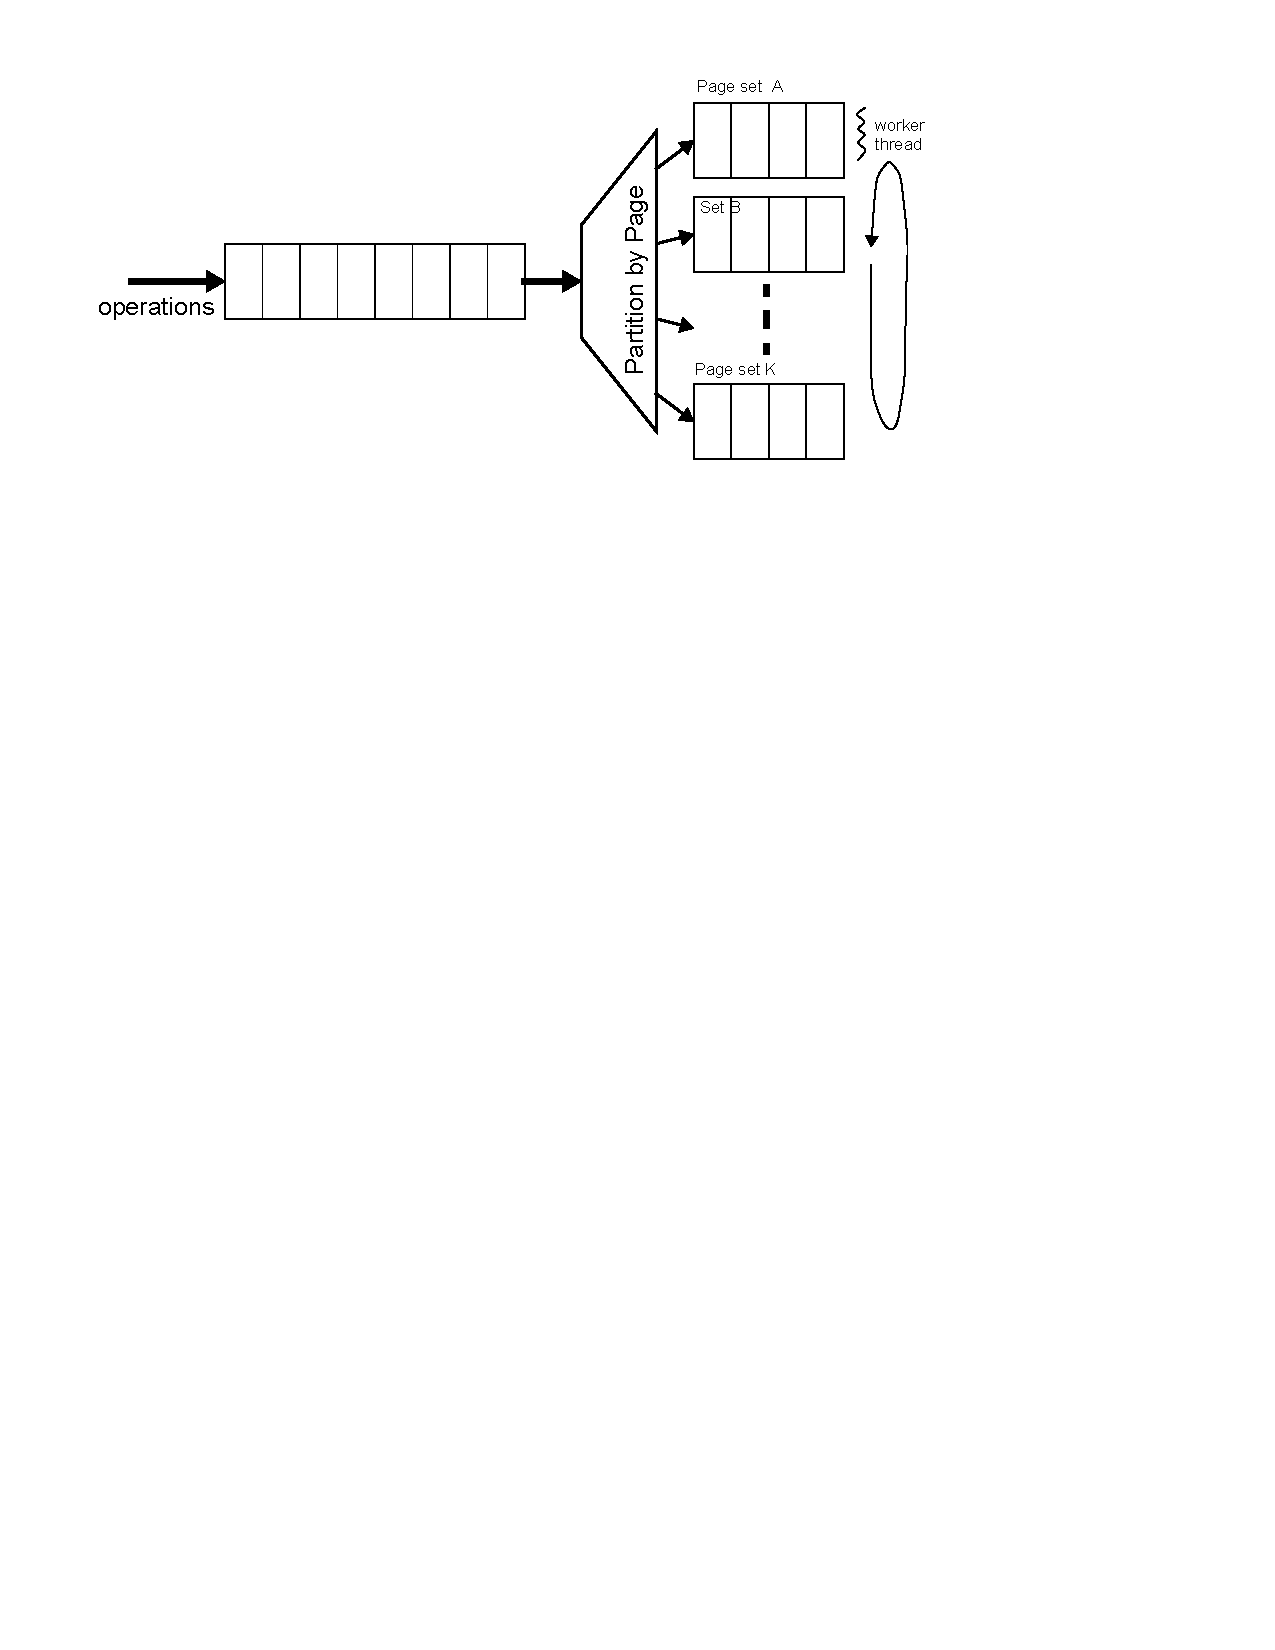
\includegraphics[width=1\columnwidth]{figs/graph-traversal.pdf}}
\vspace{-12pt}
\caption{\label{fig:multiplexor} Locality-based request reordering.
Requests are partitioned into queues.  Queue are handled
independently, improving locality and allowing requests to be merged.}
\end{figure}
\begin{figure}[t]
\graphdbg{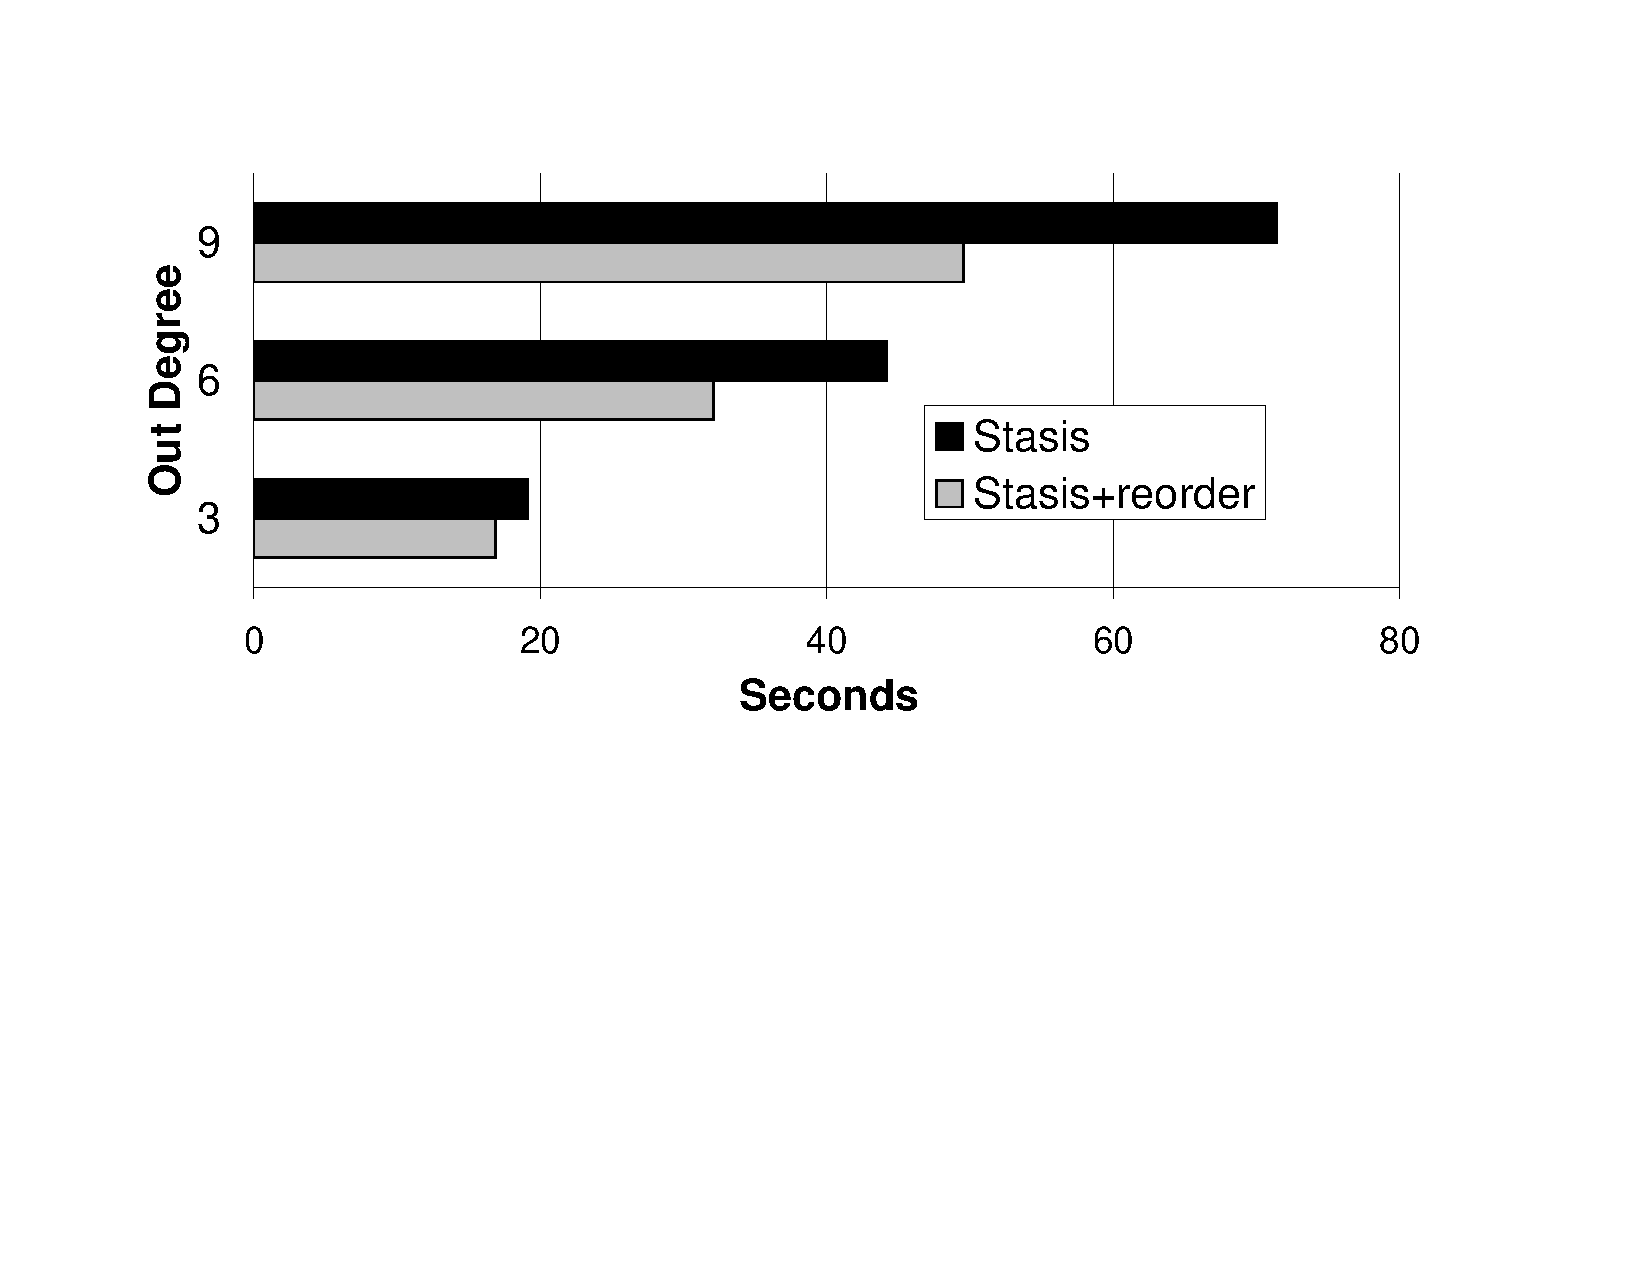
\includegraphics[%
    viewport=-13bp 19bp 600bp 280bp, 
    width=1\columnwidth]{figs/oo7.pdf}}
\vspace{-12pt}
\caption{\label{fig:oo7} OO7 benchmark style graph traversal.  The optimization performs well due to the presence of non-local nodes.}
\vspace{-12pt}
\end{figure}

\begin{figure}[t]
\graphdbg{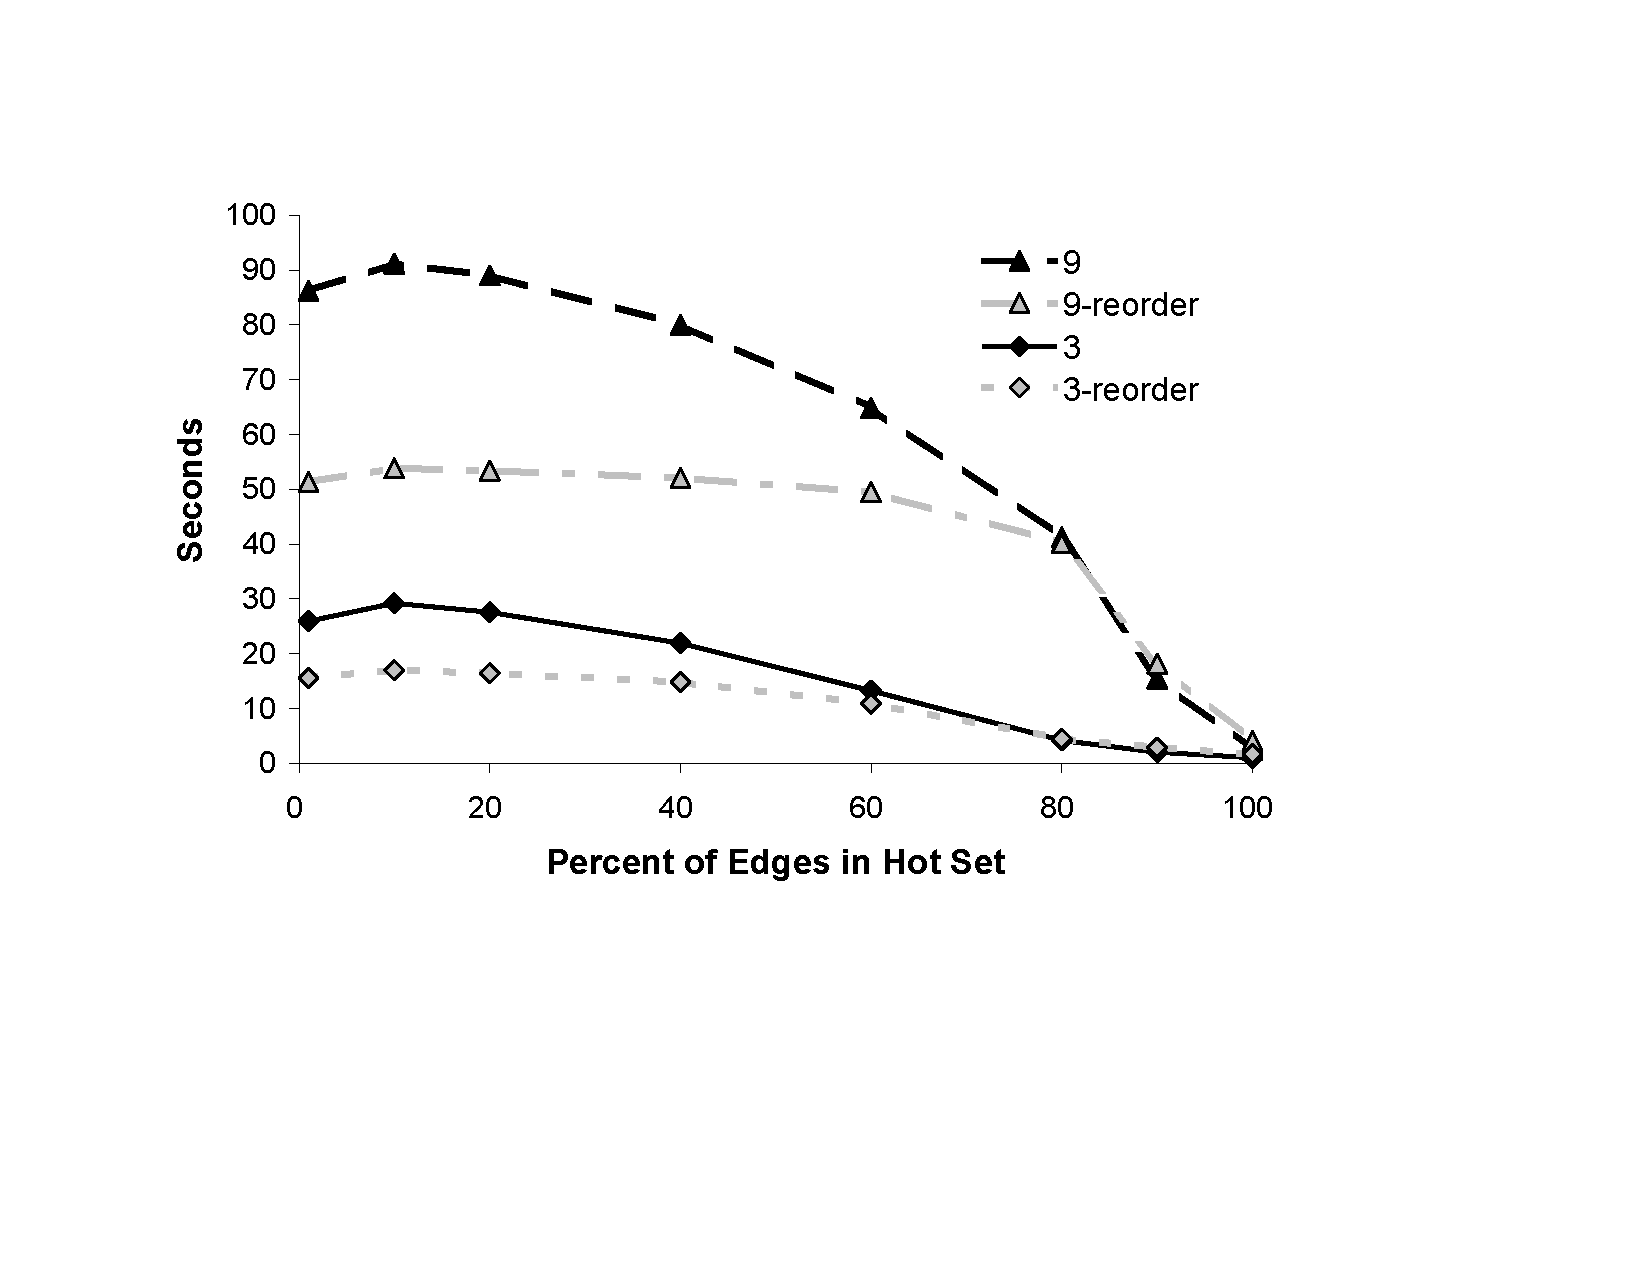
\includegraphics[%
  viewport=-5bp 15bp 525bp 336bp,
  clip,
width=1\columnwidth]{figs/trans-closure-hotset.pdf}}
\vspace{-12pt}
\caption{\label{fig:hotGraph} Hot-set based graph traversal for random graphs with out-degrees of 3 and 9.  Here
we see that the multiplexer helps when the graph has poor locality.
In the cases where depth first search performs well, the
reordering is inexpensive.}
\vspace{-12pt}
\end{figure}

We are interested in enabling \yad to manipulate sequences of
application requests.  By translating these requests into the logical
operations (such as those used for logical undo),  we can 
manipulate and optimize such requests.  Because logical operations generally
correspond to application-level operations, application developers can easily determine whether
logical operations may be reordered, transformed, or even dropped from
the stream of requests that \yad is processing.  For example,
requests that manipulate disjoint sets of data can be split across
many nodes, providing load balancing.  Requests that update the same piece of information
can be merged into a single request; RVM's ``log merging''
implements this type of optimization~\cite{lrvm}.  Stream aggregation
techniques and relational algebra operators could be used to
 transform data efficiently while it is laid out sequentially in
non-transactional memory.

To experiment with the potential of such optimizations, we implemented
a single node log-reordering scheme that increases request locality
during a graph traversal.  The graph traversal produces a sequence of
read requests that are partitioned according to their physical
location in the page file.  Partition sizes are chosen to fit inside
the buffer pool.  Each partition is processed until there are no more
outstanding requests to read from it.  The process iterates until the
traversal is complete.

We ran two experiments.  Both stored a graph of fixed-size objects in
the growable array implementation that is used as our linear
hash table's bucket list.
The first experiment (Figure~\ref{fig:oo7})
is loosely based on the OO7 database benchmark~\cite{oo7}.  We
hard-code the out-degree of each node, and use a directed graph.  Like OO7, we
construct graphs by first connecting nodes together into a ring.
We then randomly add edges until the desired
out-degree is obtained.  This structure ensures graph connectivity.
Nodes are laid out in ring order on disk so at least
one edge from each node is local.

The second experiment measures the effect of graph locality
(Figure~\ref{fig:hotGraph}).  Each node has a distinct hot set that
includes the 10\% of the nodes that are closest to it in ring order.
The remaining nodes are in the cold set.  We do not use ring edges for
this test, so the graphs might not be connected. We use the same set
of graphs for both systems.

When the graph has good locality, a normal depth-first search
traversal and the prioritized traversal both perform well.  As
locality decreases, the partitioned traversal algorithm outperforms
the naive traversal.




\section{Related Work}
\label{sec:related-work}

\subsection{Database Variations} 
\label{sec:otherDBs}

This section discusses database systems with goals similar to ours.
Although these projects were successful in many respects, each extends
the range of a fixed abstract data model.  In contrast, \yad can
support (in theory) any of these models and their extensions.

\subsubsection{Extensible databases}

Genesis is an early database toolkit that was explicitly structured in
terms of the physical data models and conceptual mappings described
above~\cite{genesis}.  It allows database implementors to swap out
implementations of the components defined by its framework.  Like
later systems (including \yad), it supports custom operations.

Subsequent extensible database work builds upon these foundations.
The Exodus~\cite{exodus} database toolkit is the successor to
Genesis. It uses abstract data type definitions, access methods and
cost models to  generate query optimizers and execution
engines automatically.

Object-oriented database systems~\cite{objectstore} and
relational databases with support for user-definable abstract data
types (such as in Postgres~\cite{postgres}) provide functionality
similar to extensible database toolkits.  In contrast to database
toolkits, which leverage type information as the database server is
compiled, object-oriented and object-relational databases allow types
to be defined at runtime.

Both approaches extend a fixed high-level data model with new
abstract data types.  This is of limited use to applications that are
not naturally structured in terms of queries over sets.

\subsubsection{Modular databases}

 The database community is also aware of this gap.  A recent
survey~\cite{riscDB} enumerates problems that plague users of
state-of-the-art database systems.  Essentially, it finds that modern
databases are too complex to be implemented or understood as a
monolithic entity.  Instead, they have become unpredictable and
unmanageable, preventing them from serving large-scale applications and
small devices.  Rather than concealing performance issues, SQL's
declarative interface prevents developers from diagnosing and
correcting underlying problems.

The study suggests that researchers and the industry adopt a highly
modular ``RISC'' database architecture.  This architecture would be
similar to a database toolkit, but would standardize the interfaces of
the toolkit's components.  This would allow competition and
specialization among module implementors, and distribute the effort
required to build a full database~\cite{riscDB}.

Streaming applications face many of the problems that RISC databases
could address.  However, it is unclear whether a single interface or
conceptual mapping would meet their needs.  Based on experiences with
their system, the authors of StreamBase argue that ``one size fits
all'' interfaces are no longer appropriate.  Instead, they argue that
the manual composition of a small number of relatively straightforward
primitives leads to cleaner, more scalable
systems~\cite{oneSizeFitsAll}.  This is in contrast to the RISC
approach, which attempts to build a database in terms of
interchangeable parts.

We agree with the motivations behind RISC databases and StreamBase,
and believe they complement each other (and \yad) well.  However, or
goal differs from these systems; we want to support applications that
are a poor fit for database systems.  However, as \yad matures we we
hope that it will enable a wide range of transactional systems,
including improved DBMSs.

\subsection{Transactional Programming Models}

\label{sec:transactionalProgramming}

Transactional programming environments provide semantic guarantees to
the programs they support.  To achieve this goal, they provide a
single approach to concurrency and transactional storage.
Therefore, they are complementary to our work; \yad provides a
substrate that makes it easier to implement such systems.

\subsubsection{Nested Transactions}

{\em Nested transactions} allow transactions to spawn sub-transactions,
forming a tree.  {\em Linear} nesting
restricts transactions to a single child.  {\em Closed} nesting rolls
children back when the parent aborts~\cite{nestedTransactionBook}.
{\em Open} nesting allows children to commit even if the parent
aborts.

Closed nesting uses database-style lock managers to allow concurrency
within a transaction.  It increases fault tolerance by isolating each
child transaction from the others, and retrying failed
transactions.  (MapReduce is similar, but uses language constructs to
statically enforce isolation~\cite{mapReduce}.)

Open nesting provides concurrency between transactions.  In
some respect, nested top actions provide open, linear nesting, as the
actions performed inside the nested top action are not rolled back
when the parent aborts.  However, logical undo gives the programmer
the option to compensate for nested top action. We expect that nested
transactions could be implemented with \yad.

\subsubsection{Distributed Programming Models}
\label{sec:argus}
%System R was one of the first relational database implementations, and
%defined a clean separation between its query processor and its storage
%subsystem.  In fact, it supported a simple navigational interface to
%the storage subsystem, which remains the architecture for modern
%databases.

Nested transactions simplify distributed systems; they isolate
failures, manage concurrency, and provide durability.  In fact, they
were developed as part of Argus, a language for reliable distributed
applications.  An Argus program consists of guardians, which are essentially
objects that encapsulate persistent and atomic data.  Accesses to {\em
atomic} data are serializable, while {\em persistent} data is atomic
data that is stored on disk~\cite{argus}.

Originally, Argus only supported limited concurrency via total
isolation, but was extended to support high concurrency data
structures.  Concurrent data structures are stored in non-atomic storage, but are augmented with
information in atomic storage.  This extra data tracks the
status of each item stored in the structure.  Conceptually, atomic 
storage used by a hash table would contain the values ``Not present'',
``Committed'' or ``Aborted; Old Value = x'' for each key in (or
missing from) the hash.  Before accessing the hash, the operation
implementation would consult the appropriate piece of atomic data, and
update the non-atomic data if necessary.  Because the atomic data is
protected by a lock manager, attempts to update the hash table are serializable.
Therefore, clever use of atomic storage can be used to provide logical locking.

Efficiently
tracking such state is not straightforward.  For example, their
hash table implementation uses a log structure to
track the status of keys that have been touched by 
active transactions.  Also, the hash table is responsible for setting 
policies regarding granularity and timing of disk writes~\cite{argusImplementation}.  \yad operations avoid this
complexity by providing logical undos, and by leaving lock management
to higher-level code.  This separates write-back and concurrency
control policies from data structure implementations.

Camelot made a number of important
contributions, both in system design, and in algorithms for
distributed transactions~\cite{camelot}.  It leaves locking to application level code,
and updates data in place.  (Argus uses shadow copies to provide
atomic updates.)  Camelot provides two logging modes: redo only
(no-steal, no-force) and undo/redo (steal, no-force).  It uses 
facilities of Mach to provide recoverable virtual memory.  It
supports Avalon, which uses Camelot to provide a
higher-level (C++) programming model.  Camelot provides a lower-level
C interface that allows other programming models to be
implemented.  It provides a limited form of closed nested transactions
where parents are suspended while children are active.  Camelot also
provides mechanisms for distributed transactions and transactional
RPC.  Although Camelot does allow applications to provide their own lock 
managers, implementation strategies for concurrent operations 
in Camelot are similar to those
built using Argus since Camelot does not provide logical undo.  Camelot focuses
on distributed transactions, and hard-codes
assumptions regarding the structure of nested transactions, consensus
algorithms, communication mechanisms, and so on.

More recent transactional programming schemes allow for multiple
transaction implementations to cooperate as part of the same
distributed transaction.  For example, X/Open DTP provides a standard
networking protocol that allows multiple transactional systems to be
controlled by a single transaction manager~\cite{dtp}.
Enterprise Java Beans is a standard for developing transactional
middle ware on top of heterogeneous storage.  Its
transactions may not be nested.  This simplifies its
semantics, and leads to many, short transactions, 
improving concurrency.  However, flat transactions are somewhat rigid, and lead to
situations where committed transactions have to be manually rolled
back by other transactions~\cite{ejbCritique}.  The Open
Multithreaded Transactions model is based on nested transactions,
incorporates exception handling, and allows parents to execute
concurrently with their children~\cite{omtt}.

QuickSilver is a distributed transactional operating system.  It
provides a transactional IPC mechanism, and
allows varying degrees of isolation, both to support legacy code, and
to implement servers that require special isolation properties.  It
supports transactions over durable and volatile state, and includes a
number of different commit protocols.  Its shared logging facility does not
hard-code log format or recovery algorithms, and supports a number
of interesting optimizations such as distributed
logging~\cite{recoveryInQuickSilver}.  The QuickSilver project found
that transactions meet the demands of most
applications, provided that long running transactions do not exhaust
system resources, and that flexible concurrency control policies are
available.  In QuickSilver, nested transactions would
be most useful when a series of program invocations
form a larger logical unit~\cite{experienceWithQuickSilver}.

\subsection{Data Structure Frameworks}

As mentioned in Section~\ref{sec:systems}, Berkeley DB is a system
quite similar to \yad, and provides raw access to
transactional data structures for application
programmers~\cite{libtp}.  \eab{summary?}

Cluster hash tables provide a scalable, replicated hash table
implementation by partitioning the table's buckets across multiple
systems~\cite{DDS}.  Boxwood treats each system in a cluster of machines as a
``chunk store,'' and builds a transactional, fault tolerant B-Tree on
top of the chunks that these machines export~\cite{boxwood}.  

\yad is complementary to Boxwood and cluster hash tables; those
systems intelligently compose a set of systems for scalability and
fault tolerance.  In contrast, \yad makes it easy to push intelligence
into the individual nodes, allowing them to provide primitives that
are appropriate for the higher-level service.  



\subsection{Data layout policies}
\label{sec:malloc}
Data layout policies make decisions based upon
assumptions about the application.  Ideally, \yad would allow
application-specific layout policies to be used interchangeably, 
This section describes strategies for data
layout that we believe \yad could eventually support.

Some large object storage systems allow arbitrary insertion and deletion of bytes~\cite{esm}
within the object, while typical file systems
provide append-only allocation~\cite{ffs}.
Record-oriented allocation, such as in VMS Record Management Services~\cite{vms} and GFS~\cite{gfs}, breaks files into addressable units.
Write-optimized file systems lay files out in the order they
were written rather than in logically sequential order~\cite{lfs}.  

Schemes to improve locality between small
objects exist as well. Relational databases allow users to specify the order
in which tuples will be laid out, and often leave portions of pages
unallocated to reduce fragmentation as new records are allocated.

Memory allocation routines such as Hoard~\cite{hoard} and
McRT-malloc~\cite{mcrt} address this problem by grouping allocated
data by thread or transaction, respectively.  This increases
locality, and reduces contention created by unrelated objects stored
in the same location.
\yads current record allocator is based on these ideas (Section~\ref{sec:locking}).

Allocation of records that must fit within pages and be persisted to
disk raises concerns regarding locality and page layouts.  Depending
on the application, data may be arranged based upon
hints~\cite{cricket}, pointer values and write order~\cite{starburst},
data type~\cite{orion}, or access
patterns~\cite{storageReorganization}.

%Other work makes use of the caller's stack to infer
%information about memory management.~\cite{xxx} \rcs{Eric, do you have
%  a reference for this?}

We are interested in allowing applications to store records in
the transaction log.  Assuming log fragmentation is kept to a
minimum, this is particularly attractive on a single disk system.  We
plan to use ideas from LFS~\cite{lfs} and POSTGRES~\cite{postgres}
to implement this.

\section{Future Work}

Complexity problems may begin to arise as we attempt to implement more
extensions to \yad.  However, \yads implementation is still fairly simple:

\begin{itemize}
\item The core of \yad is roughly 3000 lines
of C code, and implements the buffer manager, IO, recovery, and other
systems.
\item Custom operations account for another 3000 lines.
\item Page layouts and logging implementations account for 1600 lines.
\end{itemize}

The complexity of the core of \yad is our primary concern, as it
contains the hard-coded policies and assumptions.  Over time, it has
shrunk as functionality has moved into extensions.  We expect
this trend to continue as development progresses.  

A resource manager is a common pattern in system software design, and
manages dependencies and ordering constraints between sets of
components~\cite{resourceManager}.  Over time, we hope to shrink \yads core to the point
where it is simply a resource manager that coordinates interchangeable
implementations of the other components.

\section{Conclusion}

We presented \yad, a transactional storage library that addresses
the needs of system developers.  \yad provides more opportunities for
specialization than existing systems.  The effort required to extend
\yad to support a new type of system is reasonable, especially when
compared to current practices, such as working around
limitations of existing systems, breaking guarantees regarding data
integrity, or reimplementing the entire storage infrastructure from
scratch.

We demonstrated that \yad provides fully
concurrent, high-performance transactions, and explored how it can
support a number of systems that currently make use of suboptimal or
ad-hoc storage approaches.  Finally, we described how \yad can be
extended in the future to support a larger range of systems.



\section{Acknowledgements}

Thanks to shepherd Bill Weihl for helping us present these ideas well,
or at least better. The idea behind the \oasys buffer manager
optimization is from Mike Demmer; he and Bowei Du implemented \oasys.
Gilad Arnold and Amir Kamil implemented
 pobj.  Jim Blomo, Jason Bayer, and Jimmy
Kittiyachavalit worked on an early version of \yad.

Thanks to C. Mohan for pointing out that per-object LSNs may be
inadvertently overwritten during recovery.  Jim Gray suggested we use
a resource manager to track dependencies within \yad and provided
feedback on the LSN-free recovery algorithms.  Joe Hellerstein and
Mike Franklin provided us with invaluable feedback.

Portions of this work were performed at Intel Research Berkeley.

\section{Availability}
\label{sec:avail}

Additional information, and \yads source code is available at:

\begin{center}
{\small{\tt http://www.cs.berkeley.edu/\ensuremath{\sim}sears/stasis/}}
\end{center}

{\footnotesize \bibliographystyle{acm}

\rcs{Check the nocite * for un-referenced references.}
\rcs{What's ``SIGMOD International Conference on Management of Data'' vs ``SIGMOD Record''?}
\nocite{*}
\bibliography{LLADD}}

\theendnotes

\end{document}
